% % % % % % % % % % % % % % % % % % % % % % % % % % % % % % % % % % % % % % % % % % % %
%                                                                                     %
% Short Sectioned Assignment LaTeX Template Version 1.0 (5/5/12)                      %
% This template has been downloaded from: http://www.LaTeXTemplates.com               %
%                                                                                     %
% Original author:  Frits Wenneker (http://www.howtotex.com)                          %
%                                                                                     %
% Modified by: Fco Javier Sueza Rodríguez (fcosueza@disroot.org)                      %
%                                                                                     %
% Changes:                                                                            %
%	    - Custom Chapters, Sections and Subsections (titlesec package)                %
%           - Document type scrbook (oneside)                                         %
%           - Use babel-lang-spanish package and marvosym                             %
%           - Use hyperref, enumitem, tcolorbox and glossaries packages               %
%           - Use Time New Roman (mathptmx), Helvetic and Courier fonts               %
%                                                                                     %
% License: CC BY-NC-SA 3.0 (http://creativecommons.org/licenses/by-nc-sa/3.0/)        %
%                                                                                     %
% % % % % % % % % % % % % % % % % % % % % % % % % % % % % % % % % % % % % % % % % % % %

%-----------------------------------------------%
%	              Packages                  %
%-----------------------------------------------%

\documentclass[paper=a4, fontsize=11pt, oneside]{scrbook}

% ---- Text Input/Output ----- %

\usepackage[T1]{fontenc}
\usepackage[utf8]{inputenc}
\usepackage{mathptmx}
\usepackage[scaled=.92]{helvet}
\usepackage{courier}
\usepackage[indent=12pt]{parskip}

\usepackage{geometry}
\geometry{verbose,tmargin=3cm,bmargin=3cm,lmargin=2.6cm,rmargin=2.6cm}

% ---- Language ----- %

\usepackage[spanish]{babel}
\usepackage{marvosym}

% ---- Another packages ---- %

\usepackage{amsmath,amsfonts,amsthm}
\usepackage{graphics,graphicx}
\usepackage{titlesec}
\usepackage{fancyhdr}
\usepackage{tcolorbox}
\usepackage{hyperref}
\usepackage{enumitem}
\usepackage[automake]{glossaries}

%--------------------------------------------------------------------%
%                      Customizing Document                          %
%--------------------------------------------------------------------%


% ----------- Custom Chapters, Sections and Subsections -------------- %

\titleformat{\chapter}[display]
			{\bfseries\Huge}
			{Tema \ \thechapter} {0.5ex}
			{\vspace{1ex}\centering}

\titleformat{\section}[hang]
			{\bfseries\Large}
			{\thesection}{0.5em}{}

\titleformat{\subsection}[hang]
			{\bfseries\large}
			{\thesubsection}{0.5em}{}

\titleformat{\subsubsection}[hang]
			{\bfseries\large}
			{\thesubsubsection}{0.5em}{}

\hypersetup{
    colorlinks=true,
    linkcolor=black,
    urlcolor=magenta
}

% ------------------- Custom heaaders and footers ------------------- %

\pagestyle{fancyplain}

\fancyhead[]{}
\fancyfoot[L]{}
\fancyfoot[C]{}
\fancyfoot[R]{\thepage}

\renewcommand{\headrulewidth}{0pt} % Remove header underlines
\renewcommand{\footrulewidth}{0pt} % Remove footer underlines

\setlength{\headheight}{13.6pt} % Customize the height of the header

% --------- Numbering equations, figures and tables ----------------- %

\numberwithin{equation}{section} % Number equations within sections
\numberwithin{figure}{section} % Number figures within sections
\numberwithin{table}{section} % Number tables within sections

% ------------------------ New Commands ----------------------------- %

\newcommand{\horrule}[1]{\rule{\linewidth}{#1}} % Create horizontal rule command


%----------------------------------------------------------------------------------------
%	TÍTULO Y DATOS DEL ALUMNO
%----------------------------------------------------------------------------------------

\title{
    \vspace{10ex}
    \normalfont \normalsize
    \huge \textbf{Actividades de la Unidad 2}
}
\author{Francisco Javier Sueza Rodríguez}
\date{\normalsize\today}

%----------------------------------------------------------------------------------------
%                                     DOCUMENTO
%----------------------------------------------------------------------------------------
\begin{document}

\maketitle

\thispagestyle{empty}

\vspace{75ex}

\begin{center}
    \begin{tabular}{l l}
        \textbf{Centro}: & IES Aguadulce \\
        \textbf{Ciclo Formativo}: & Desarrollo Aplicaciones Web (Distancia)\\
        \textbf{Asignatura}: & Entornos de Desarrollo\\
       \textbf{Tema}: & Tema 2 - Desarrollo de Software y Entornos de Desarrollo\\
    \end{tabular}
\end{center}

\newpage

\tableofcontents

\newpage

\vspace{2.5ex}

\listoffigures

\newpage

\section{Caso Práctico}
La empresa SOFTED ha recibido un nuevo encargo de software

En esta ocasión, todo el software que se desarrolle debería estar integrado en algún entorno de desarrollo libre. Ada ha elegido trabajar con NetBeans y utilizar como sistema operativo Windows o Linux.

Una vez planteado el análisis de requerimientos y el diseño de la aplicación (tal y como hicimos en la unidad anterior), se requiere tener un buen entorno para el diseño y ejecución de los programas.

- Venga, no te agobies, vamos a echar un café y nos ponemos manos a la obra,...- insiste Juan.

\section{Actividades}
En esta tarea vamos a realizar la instalación y configuración de \textbf{Netbeans 14}, así como ver un ejemplo de uso con una aplicación sencilla realizada en Java. Para esto, será también necesario la instalación del SDK de Java, en nuestro caso instalaremos la versión \textbf{JDK SE 11.0.13}, que realizaremos en primer lugar y antes de la instalación de Netbeans.

Además, en último lugar se instalará \textbf{Intellij IDEA}, para probar otro IDE a parte de Netbeans.

\subsection{Actividad 1}

\subsubsection{Enunciado}
Vamos a instalar el IDE Netbeans. Para ello se instalará por separado el JDK SE 11.0.13 y el IDE NetBeans 14. Puedes encontrar ambos archivos desde los enlaces del apartado 2.- Información de interés.

\begin{enumerate}[label=(\alph*)]
    \item Para la instalación de JDK cambia la carpeta de destino de instalación añadiendo una subcarpeta llamada XXX2223 (donde XXX sean tus iniciales), quedando la ruta: C:\textbackslash Program Files\textbackslash Java\textbackslash jdk-11.0.13\textbackslash XXX2223\ (para este apartado debes entregar dos capturas, la que muestra la carpeta de destino de la instalación con las modificaciones solicitadas y la captura de la última ventana que muestra que se ha finalizado la instalación correctamente).
    \item Para la instalación de Netbeans cambia la carpeta de destino de instalación añadiendo un subcarpeta llamada XXX2223 (donde XXX sean tus iniciales), quedando la ruta: C:\textbackslash Program File\textbackslash NetBeans-14\textbackslash XXX2223\ y el JDK instalado en el apartado anterior (para este apartado debes entregar otras dos capturas, la que se muestra en la carpeta de destino de la instalación con las modificaciones solicitadas y la captura de la última ventana que muestra que se ha finalizado la instalación correctamente).

    Capturas solicitadas: 4 (dos por cada apartado).
    \begin{itemize}
        \item Captura de pantalla donde se vea la instalación de JDK en la ruta indicada.
        \item Captura desde el símbolo del sistema donde se vea la versión instalada de JDK (para poder verlo escribimos en la consola: java -version)
        \item Captura mientras se instala NetBeans donde se vea la ruta de instalación indicada.
        \item Captura mostrando que el proceso de instalación ha finalizado correctamente.
    \end{itemize}
\end{enumerate}

\subsubsection{Solución}
En primer lugar vamos a instalar \textbf{JDK SE 13.0.11} y \textbf{Netbeans 14}. Hay que tener en cuenta que vamos a instalarlos \textbf{por separado} por lo que no nos vale el bundle que podemos encontrar donde Netbeans ya incluye el JDK en cuestión.

\begin{enumerate}[label=(\alph*)]
    \item Primeramente vamos a instalar el JDK solicitado. Podemos descargarlo desde la \href{https://www.oracle.com/java/technologies/javase/jdk13-archive-downloads.html}{página oficial de Oracle} dedicada a las versiones antiguas. Una vez descargado ejecutamos el instalador y comenzamos el proceso de instalación. Nosotros hemos elegido como \textbf{directorio de instalación} la ruta \textbf{C:\textbackslash Program Files\textbackslash Java\textbackslash jdk-11.0.13\textbackslash FJS2223\ }, como se pide en el enunciado usando nuestras iniciales, como se puede ver en la siguiente captura.

    \begin{figure}[ht]
        \centering
        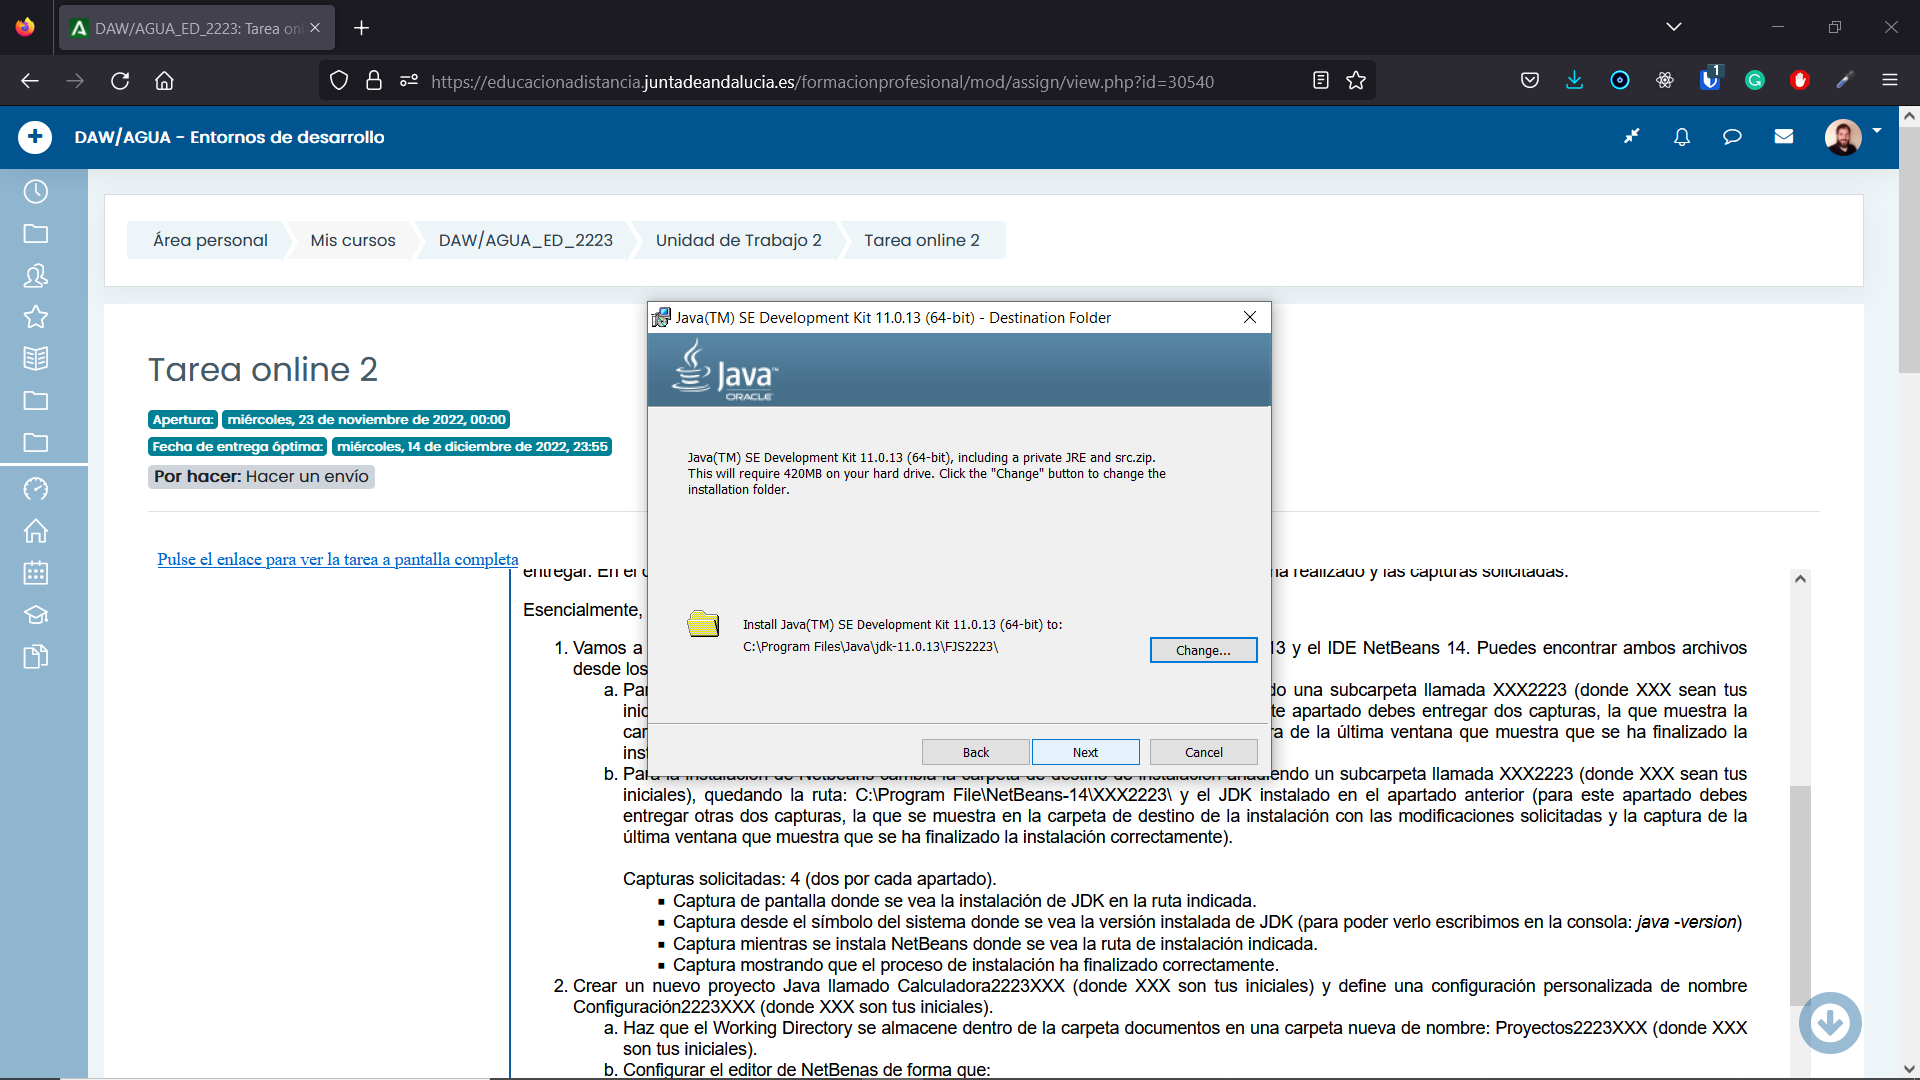
\includegraphics[scale=0.32]{jdk-install-1.png}
        \caption{Instalador de JDK y selección de directorio}
    \end{figure}

    Una vez seleccionado el directorio de instalación, ésta ha continuado con normalidad y se ha completado, como se muestra en la siguiente figura.

    \begin{figure}[ht]
        \centering
        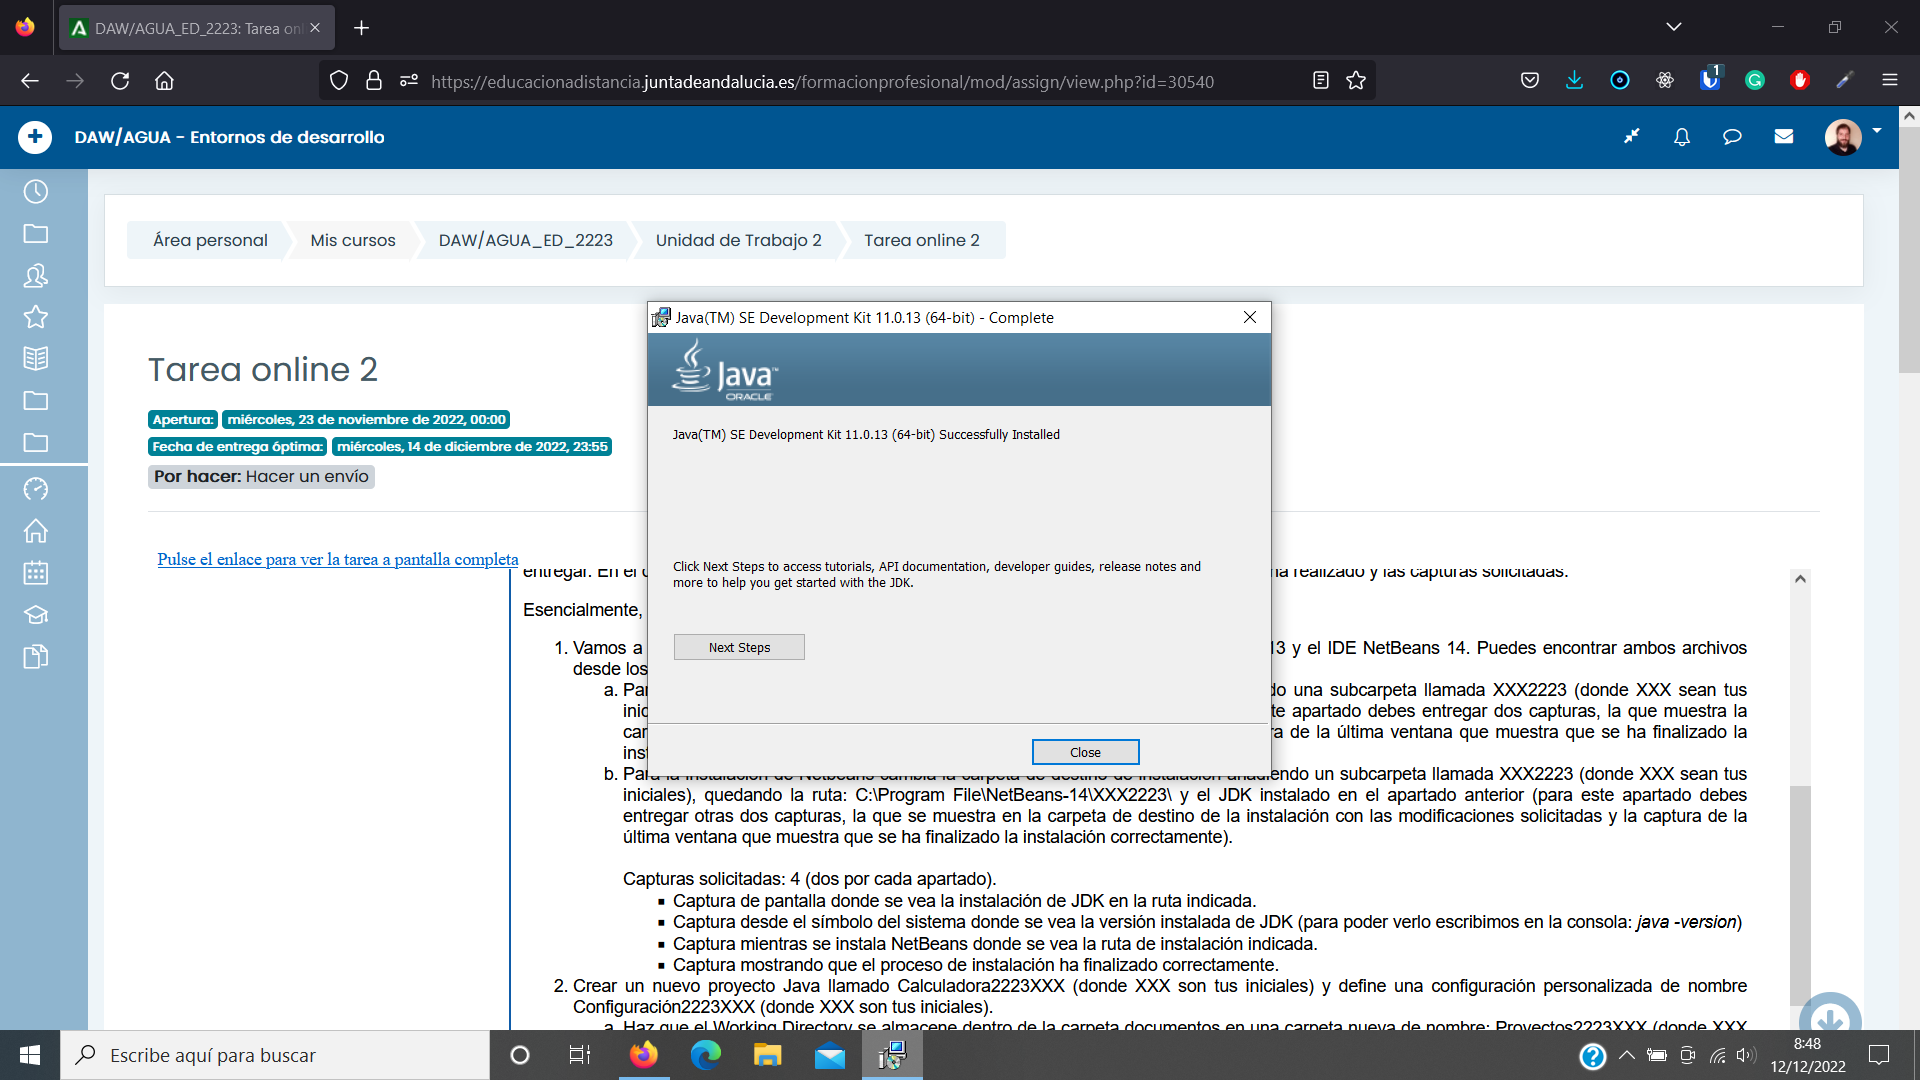
\includegraphics[scale=0.32]{jdk-install-2.png}
        \caption{Instalación de JDK SE completada}
    \end{figure}

    Para asegurarnos de que la instalación se ha realizado correctamente y la versión es la adecuada lo hemos comprobado desde la consola de Windows, usando el comando \textbf{``java --version''}.

    \begin{figure}[ht]
        \centering
        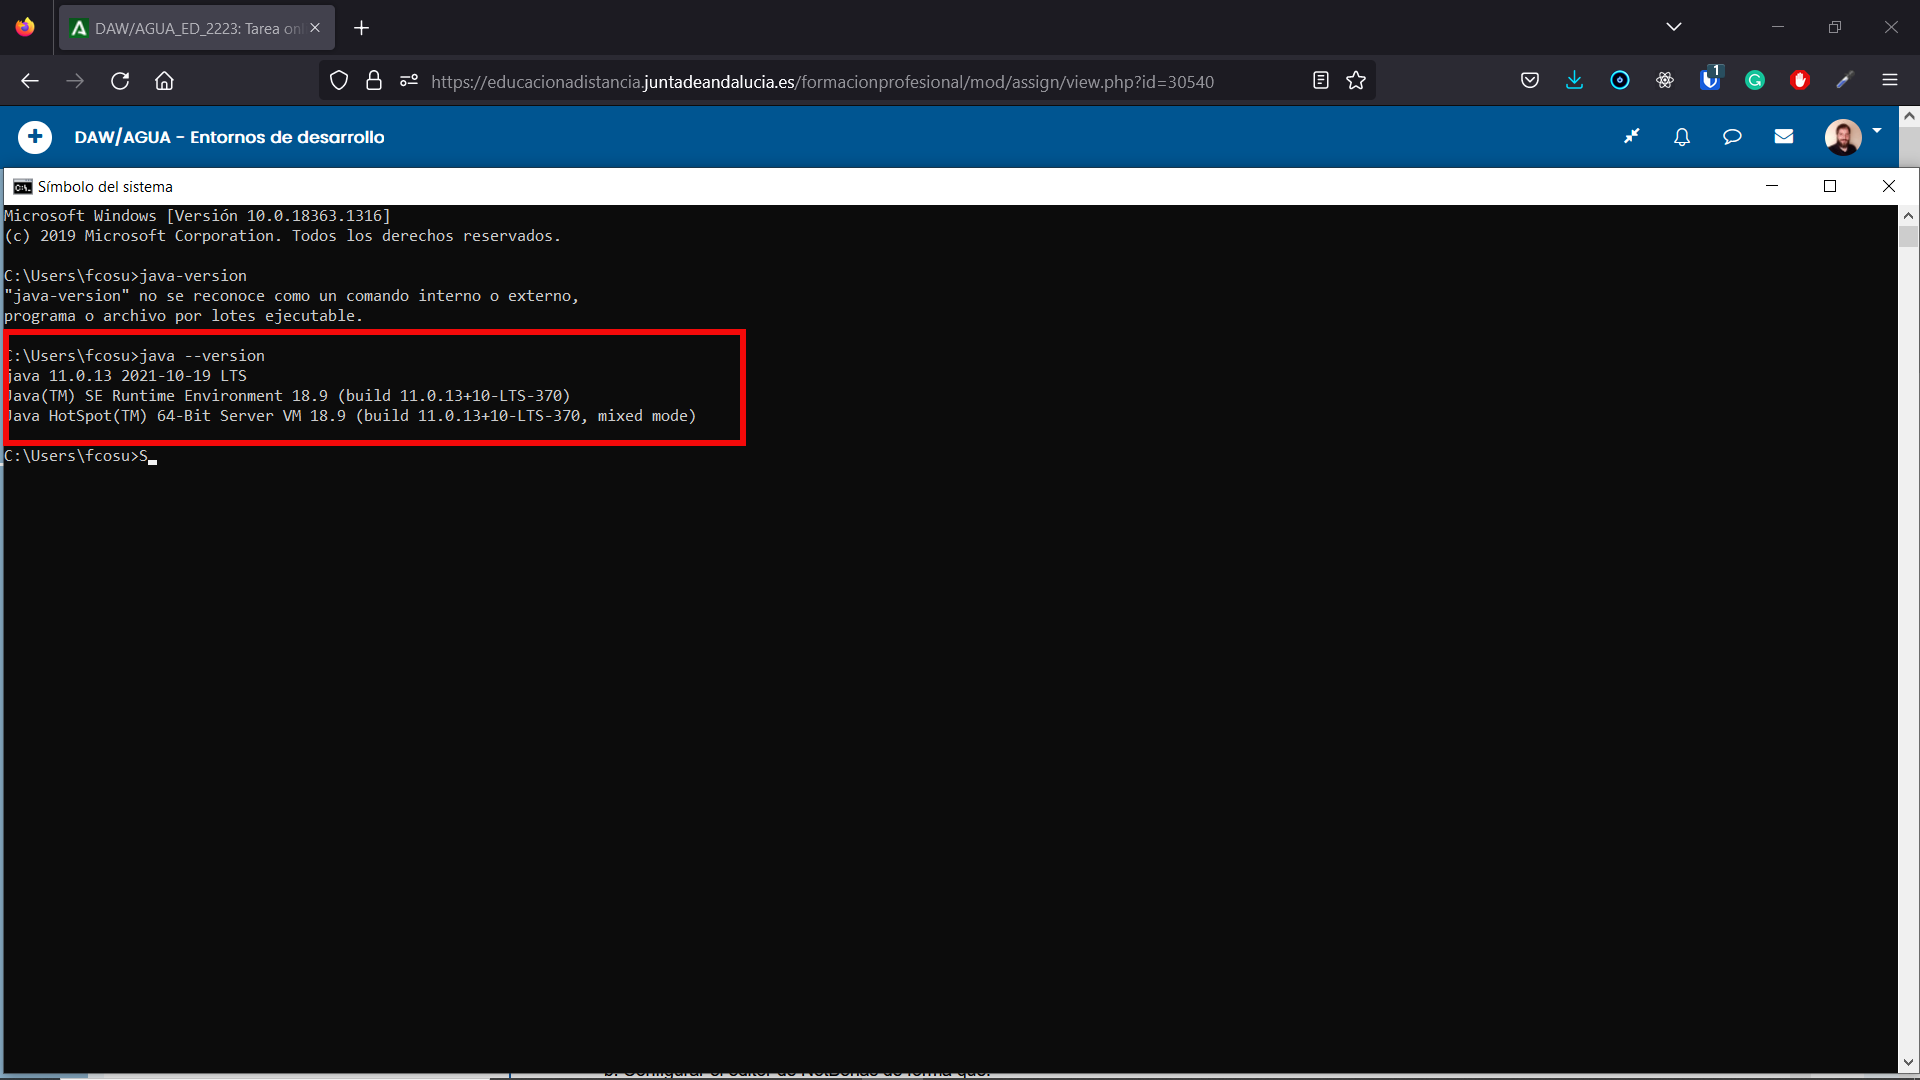
\includegraphics[scale=0.32]{jdk-install-3.png}
        \caption{Comprobación de versión de JDK instalada}
    \end{figure}

    \item A continuación hemos instalado \textbf{Netbeans 14}, descargando el instalador desde la \href{https://netbeans.apache.org/download/nb14/}{página oficial de netbeans}. Una vez ejecutado el instalador, se nos pide que seleccionemos los complementos a instalar, que nosotros hemos seleccionado por defecto. También se nos pedirá que especifiquemos la ruta del JDK instalado, aunque por norma general suele estar seleccionada la correcta por defecto.

     En la siguiente pantalla hemos cambiado el directorio de instalación al siguiente: \textbf{C:\textbackslash Program Files\textbackslash Netbeans-14\textbackslash FJS2223\ }.

    \begin{figure}[ht]
        \centering
        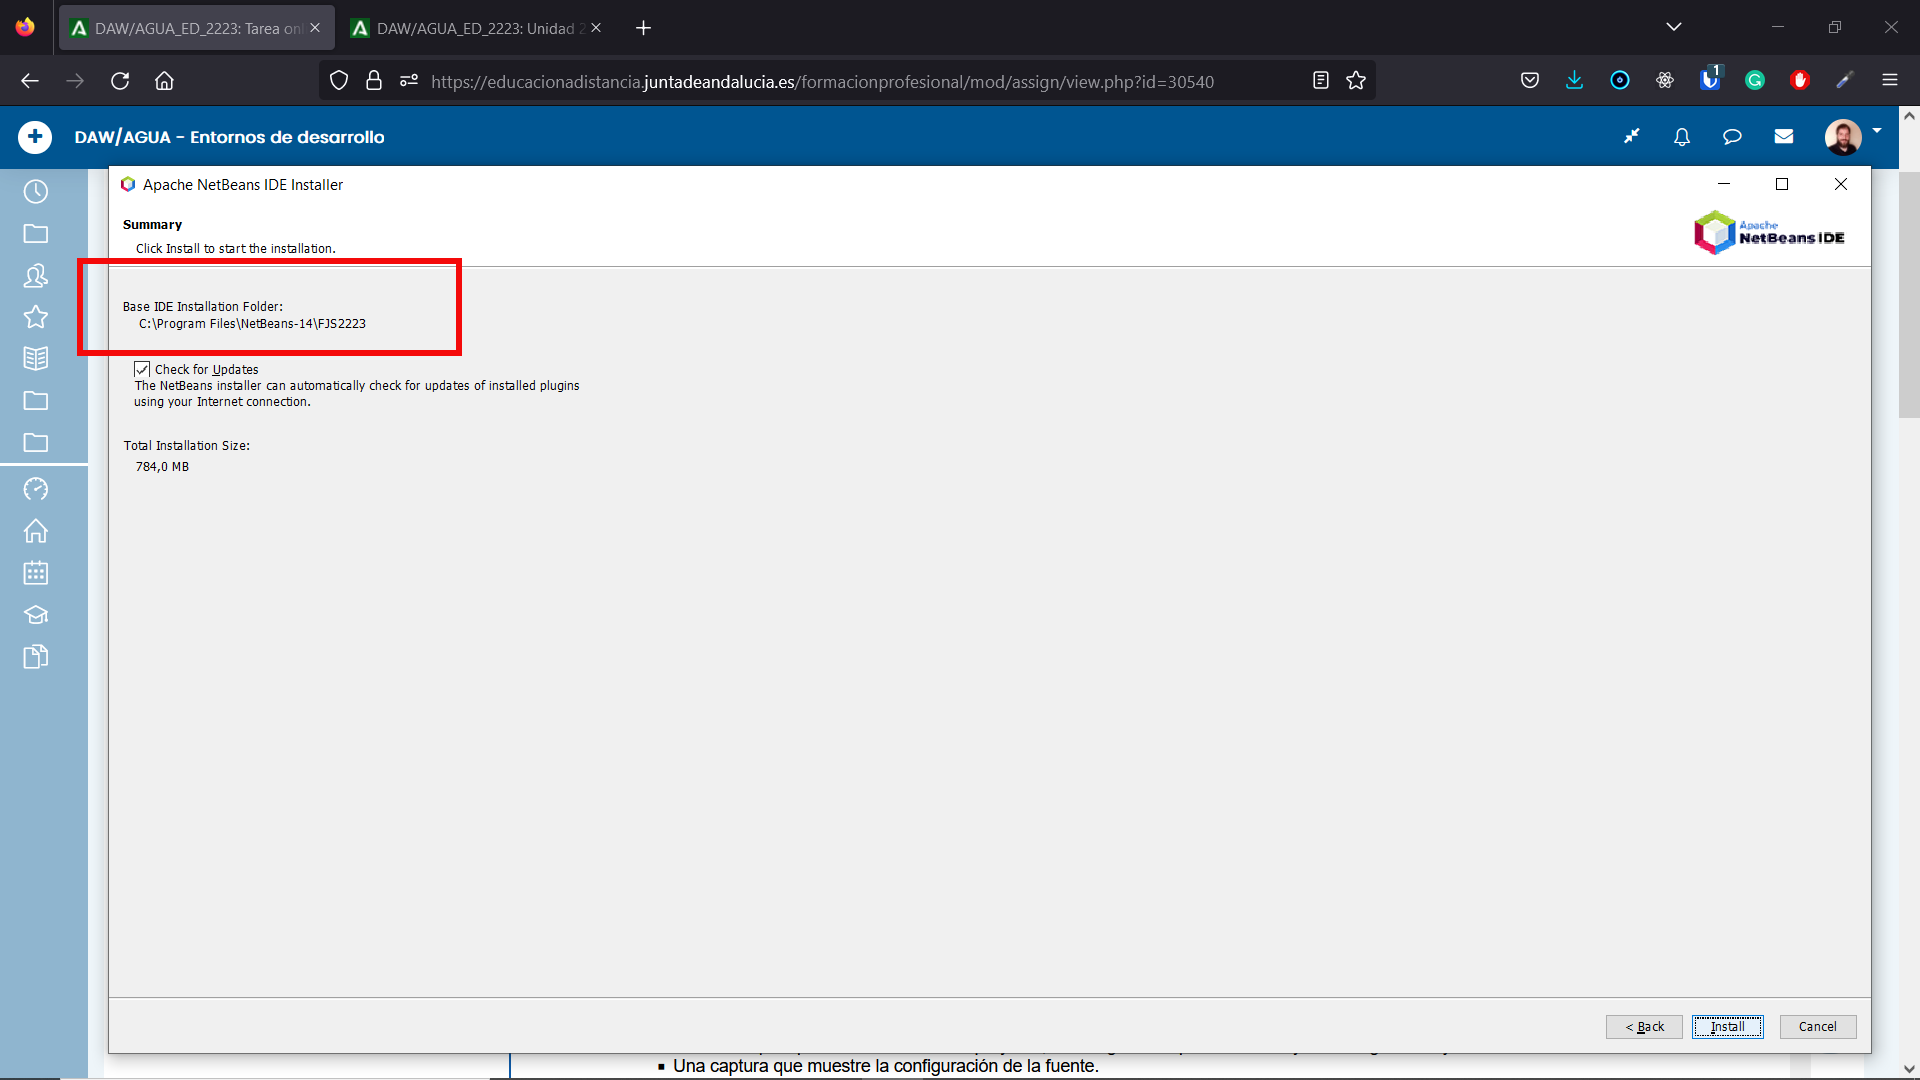
\includegraphics[scale=0.32]{netbeans-install-1.png}
        \caption{Instalador de Netbeans y selección de directorio}
    \end{figure}

    Después de seleccionar el directorio, hemos procedido con la instalación, la cual se ha realizado con éxito.

    \begin{figure}[ht]
        \centering
        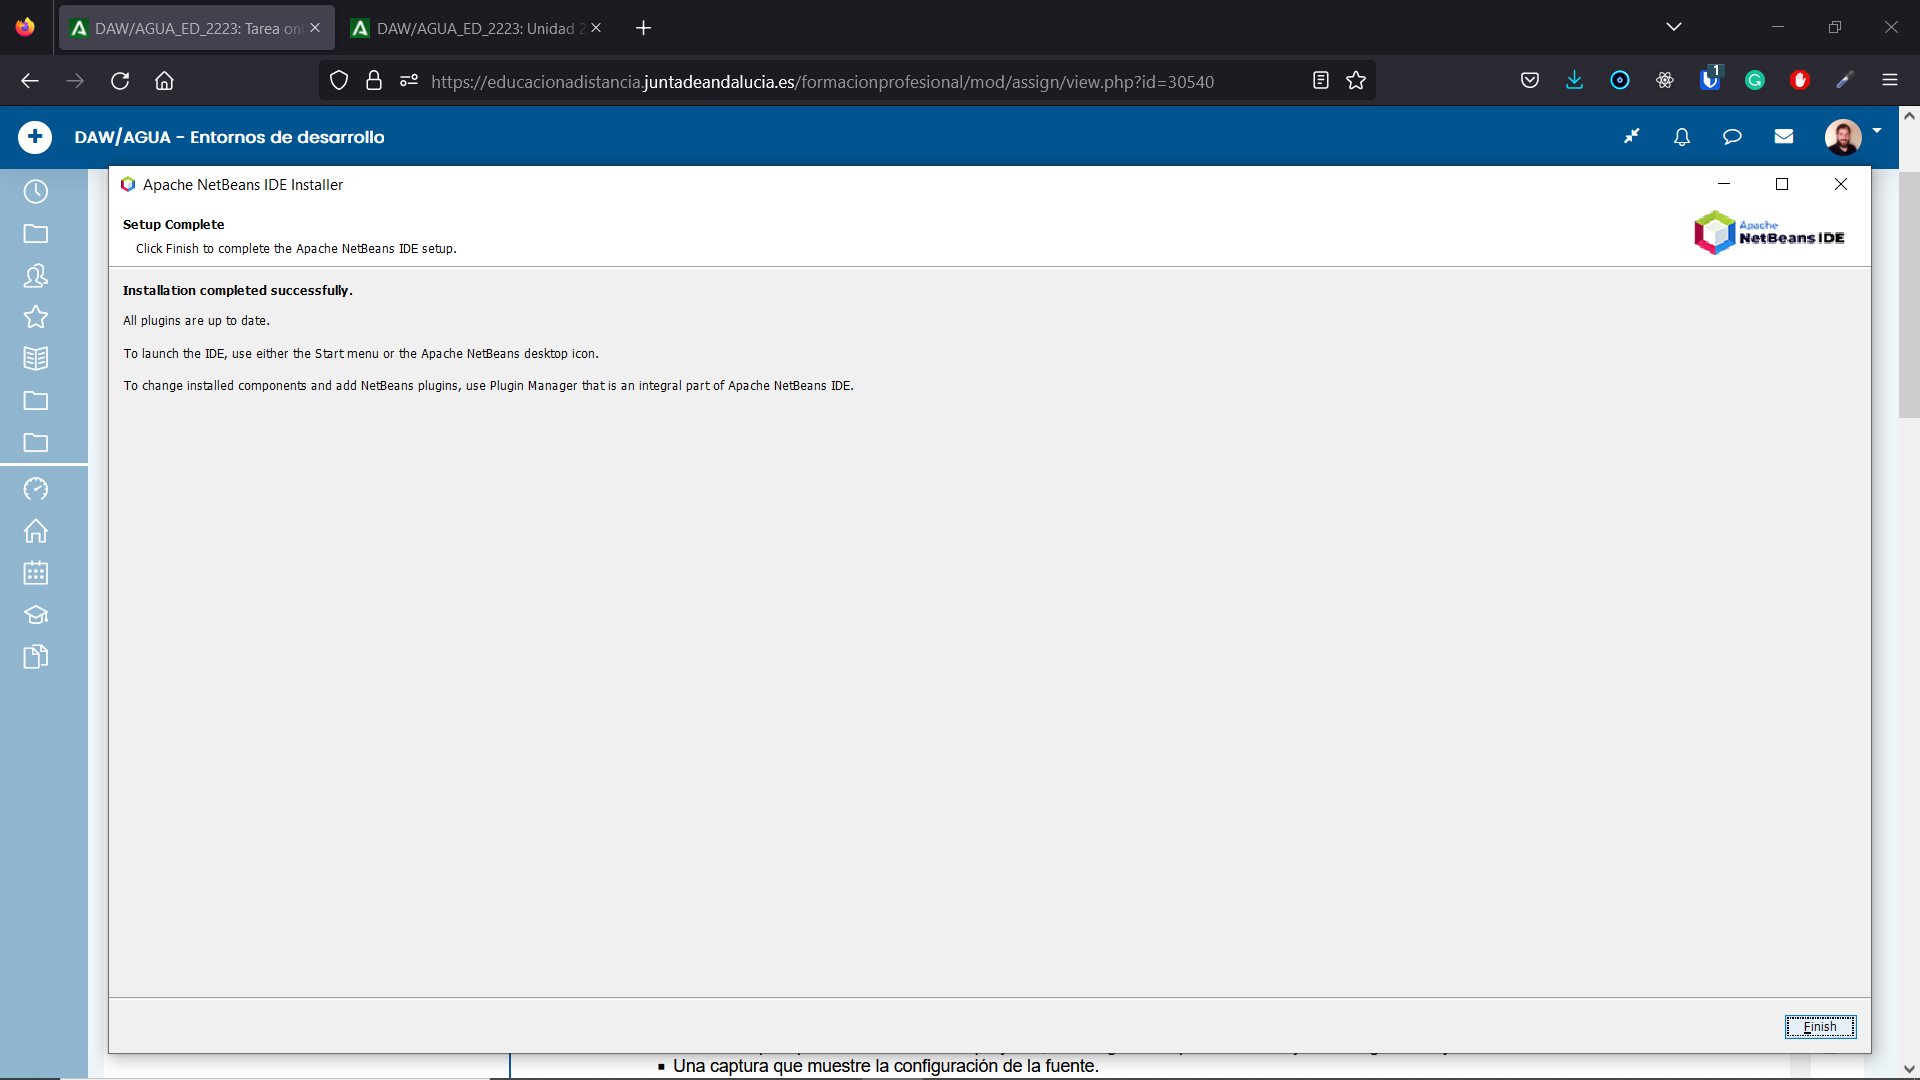
\includegraphics[scale=0.32]{netbeans-install-2.png}
        \caption{Instalación de Netbeans completada}
    \end{figure}
\end{enumerate}

\subsection{Actividad 2}
\subsubsection{Enunciado}
Crear un nuevo proyecto Java llamado Calculadora2223XXX (donde XXX son tus iniciales) y define una configuración personalizada de nombre Configuración2223XXX (donde XXX son tus iniciales).

\begin{enumerate}[label=(\alph*)]
    \item Haz que el Working Directory se almacene dentro de la carpeta documentos en una carpeta nueva de nombre: Proyectos2223XXX (donde XXX son tus iniciales).

    \item Configurar el editor de NetBenas de forma que:
    \begin{itemize}
        \item La fuente sea Arial 12 en azul
        \item Los Warning aparezcan con el texto en color naranja y negrita.
    \end{itemize}

    Capturas solicitadas: 3
    \begin{itemize}
        \item Una en la que aparezca el nombre del proyecto, la configuración personalizada y el woking directory.
        \item Una captura que muestre la configuración de la fuente.
        \item Una captura que muestre la configuración de los warning.
    \end{itemize}
\end{enumerate}

\subsubsection{Solución}
En este punto vamos a crear un nuevo proyecto en Netbeans y realizar algunas configuraciones básicas, creando una configuración personalizada.

\begin{enumerate}[label=(\alph*)]
    \item En primer lugar hemos creado el proyecto, con nombre \textbf{Calculadora2223FJS} y hemos definido una configuración personalizada. Esto lo podemos hacer pulsando con el botón derecho sobre el nombre del proyecto y seleccionando la opción \textit{``Preferences''}. En la ventana que se nos abre, en el aparado \textit{``Run''} podemos realizar lo cambios requeridos para este punto. Hemos creado un nuevo archivo de configuración personalizado con el nombre \textbf{Configuracion2223FJS} y se ha cambiado el \textbf{Working Directory} a \textbf{C:\textbackslash Users\textbackslash fcosu\textbackslash Documents\textbackslash Proyectos2223FJS }.

    \begin{figure}[ht]
        \centering
        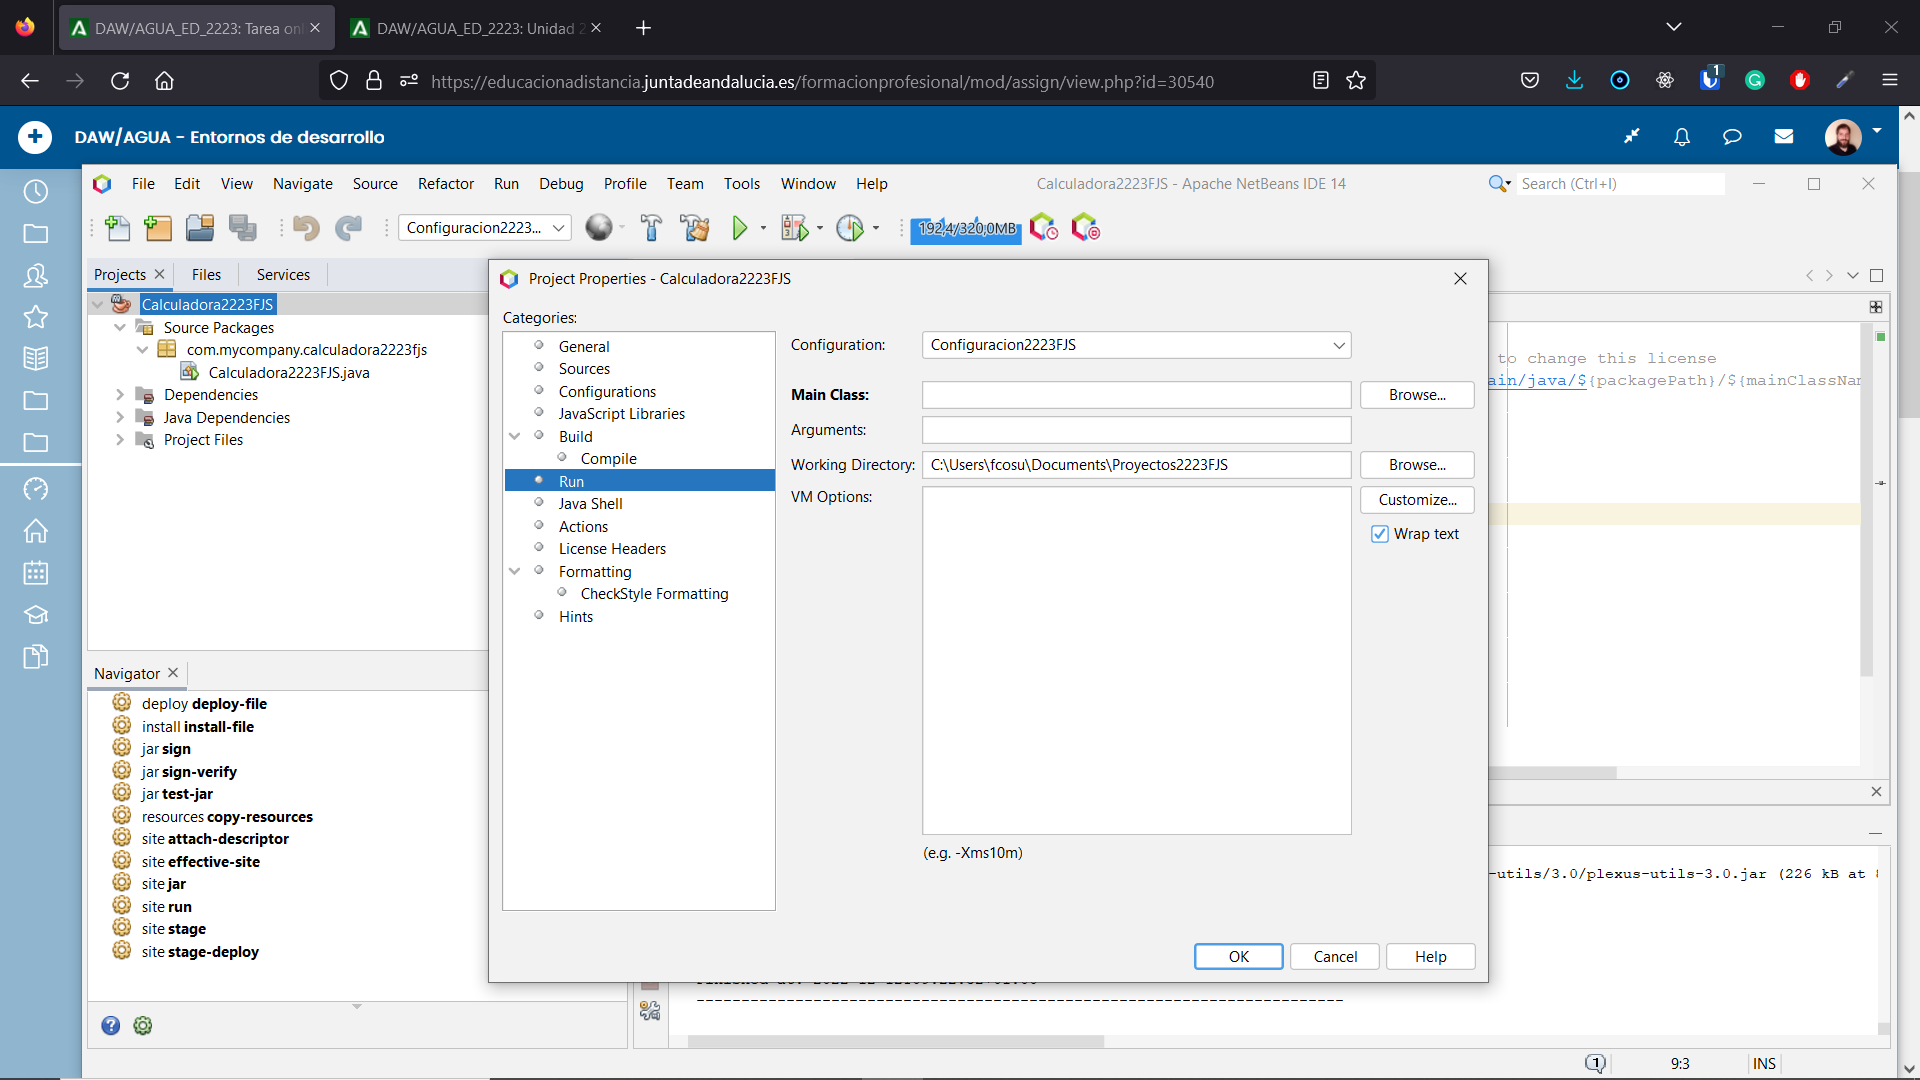
\includegraphics[scale=0.32]{netbeans-config-1.png}
        \caption{Configuración de Netbeans}
    \end{figure}

    \item A continuación hemos cambiado de sección a \textit{``Formating''} en la misma pantalla de preferencias. Ahí, hemos pulsado en la opción \textit{``Edit Global Options''}. Esto nos abrirá una nueva ventana, donde pulsaremos en la pestaña \textit{``Fonts \& Color''} para poder cambiar el color y el tipo del \textbf{texto principal} de Netbeans, que hemos elegido el tipo Arial de color azul..

     \begin{figure}[ht]
        \centering
        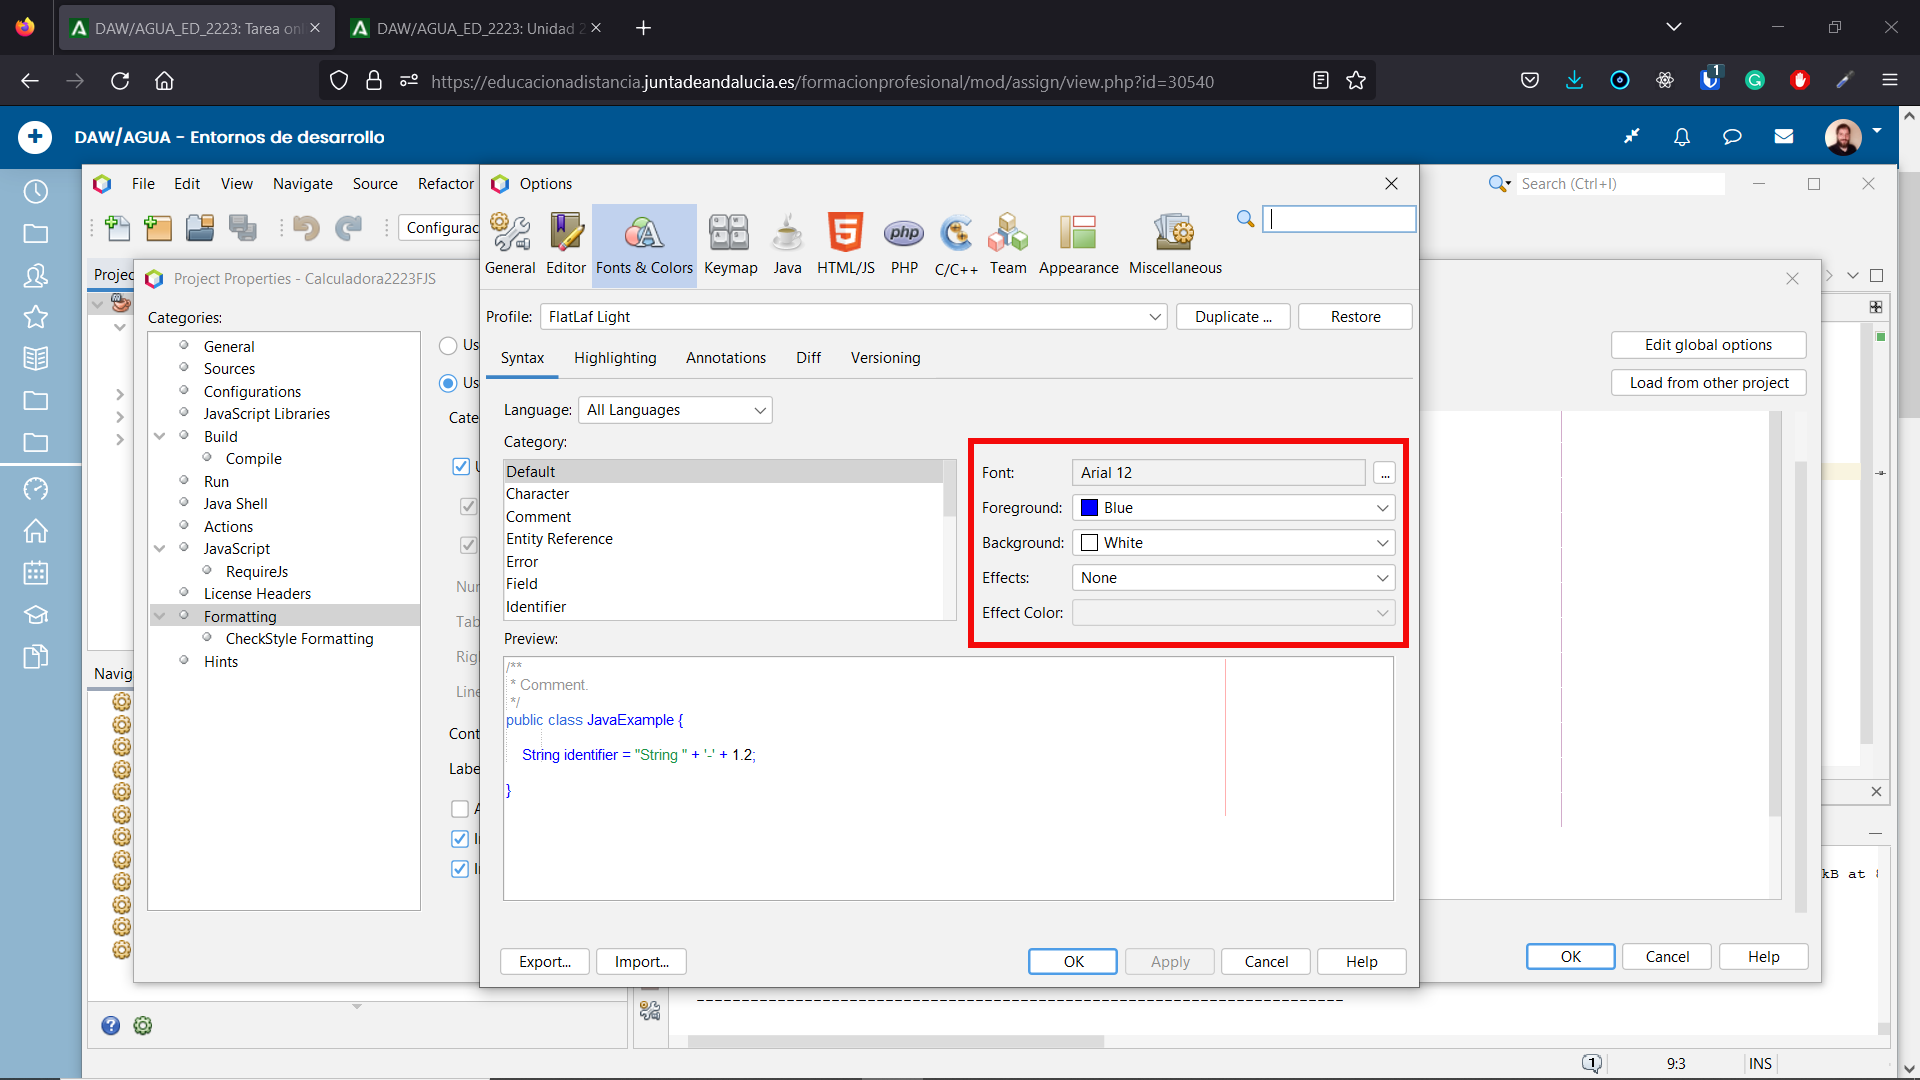
\includegraphics[scale=0.32]{netbeans-config-2.png}
        \caption{Cambio del tipo y color de letra del editor}
    \end{figure}

     También se puede cambiar el color de diferentes tokens o elementos concretos, en este caso, solo hemos cambiado los \textbf{mensajes de Warning} a color naranja. En la siguiente figura se muestra el cambio de este elemento.

   \begin{figure}[ht]
       \centering
       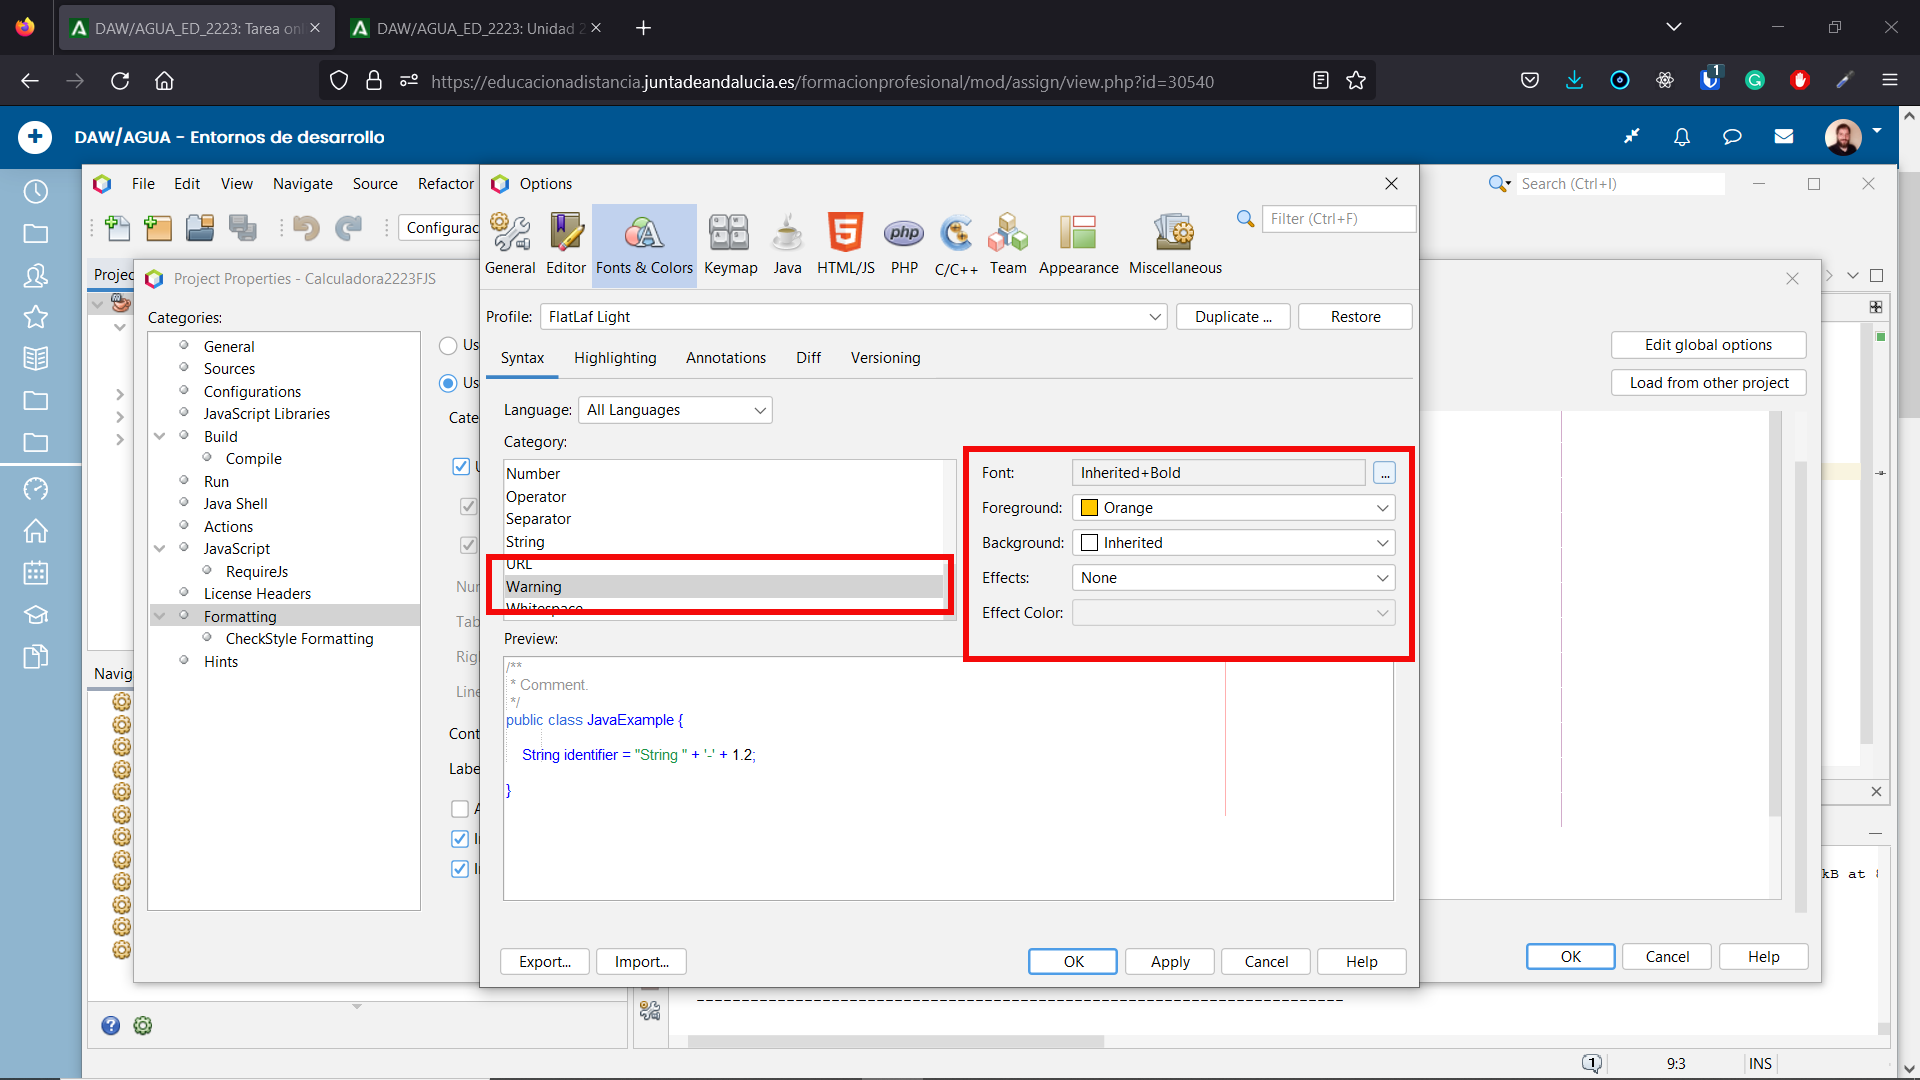
\includegraphics[scale=0.32]{netbeans-config-3.png}
       \caption{Cambio del color y resaltado de los mensajes de Warning}
    \end{figure}
\end{enumerate}

\subsection{Actividad 3}
\subsubsection{Enunciado}
Instala los plugin NB Java Decompiler de forma off-line y Explore Location in OS de forma on-line.

Capturas solicitadas: 4 (dos por cada plugin)
\begin{itemize}
    \item Una captura que muestre el plugin NB Java Decompiler se está instalando de forma off-line desde el IDE.
    \item Una captura que muestre que el plugin NB Java Decompiler ha finalizado la instalación correctamente.
    \item Una captura que muestre que el plugin Explore Location in OS se está instalando de forma on-line desde el IDE.
    Una captura que muestre que el plugin Explore Location in OS ha finalizado la instalación correctamente.
\end{itemize}

\subsubsection{Solución}
En esta actividad vamos a instalar dos plugins de Netbeans. El primero será \textbf{NB Java Decompiler}, que instalaremos de forma \textbf{off-line} y en segundo lugar instalaremos \textbf{Explore Location OS}, que instalaremos de forma \textbf{on-line}.

\begin{itemize}
    \item Para instalar de forma \textbf{off-line} un plugin de Netbeans debemos descargarlo nosotros manualmente y después cargarlo desde el IDE. Hemos descargado \textbf{NB Java Decompile} desde la \href{https://plugins.netbeans.apache.org/catalogue/?id=80}{página oficial de plugins de Netbeans}. Una vez descargado, pulsamos en el menú \textit{``Tools''} y ahí en la opción \textit{``Plugins''}.

    En la ventana que se nos abrirá debemos seleccionar la pestaña \textit{``Downloaded''}, que nos permitirá cargar e instalarlo, como se puede ver en las siguientes capturas. Una vez instalado, el plugin desaparecerá de esa pestaña y aparecerá en la pestaña \textit{``Ìnstalled''}.

    Es posible que durante el proceso de instalación se nos muestre una \textbf{ventana con una advertencia}, si por lo que sea algún plugin aparece como no firmado. En principio si el plugin está descargado desde un sitio oficial, como es el caso, no deberíamos preocuparnos. Podemos cerrar la ventana y continuar con el proceso de instalación.

    \begin{figure}[H]
        \centering
        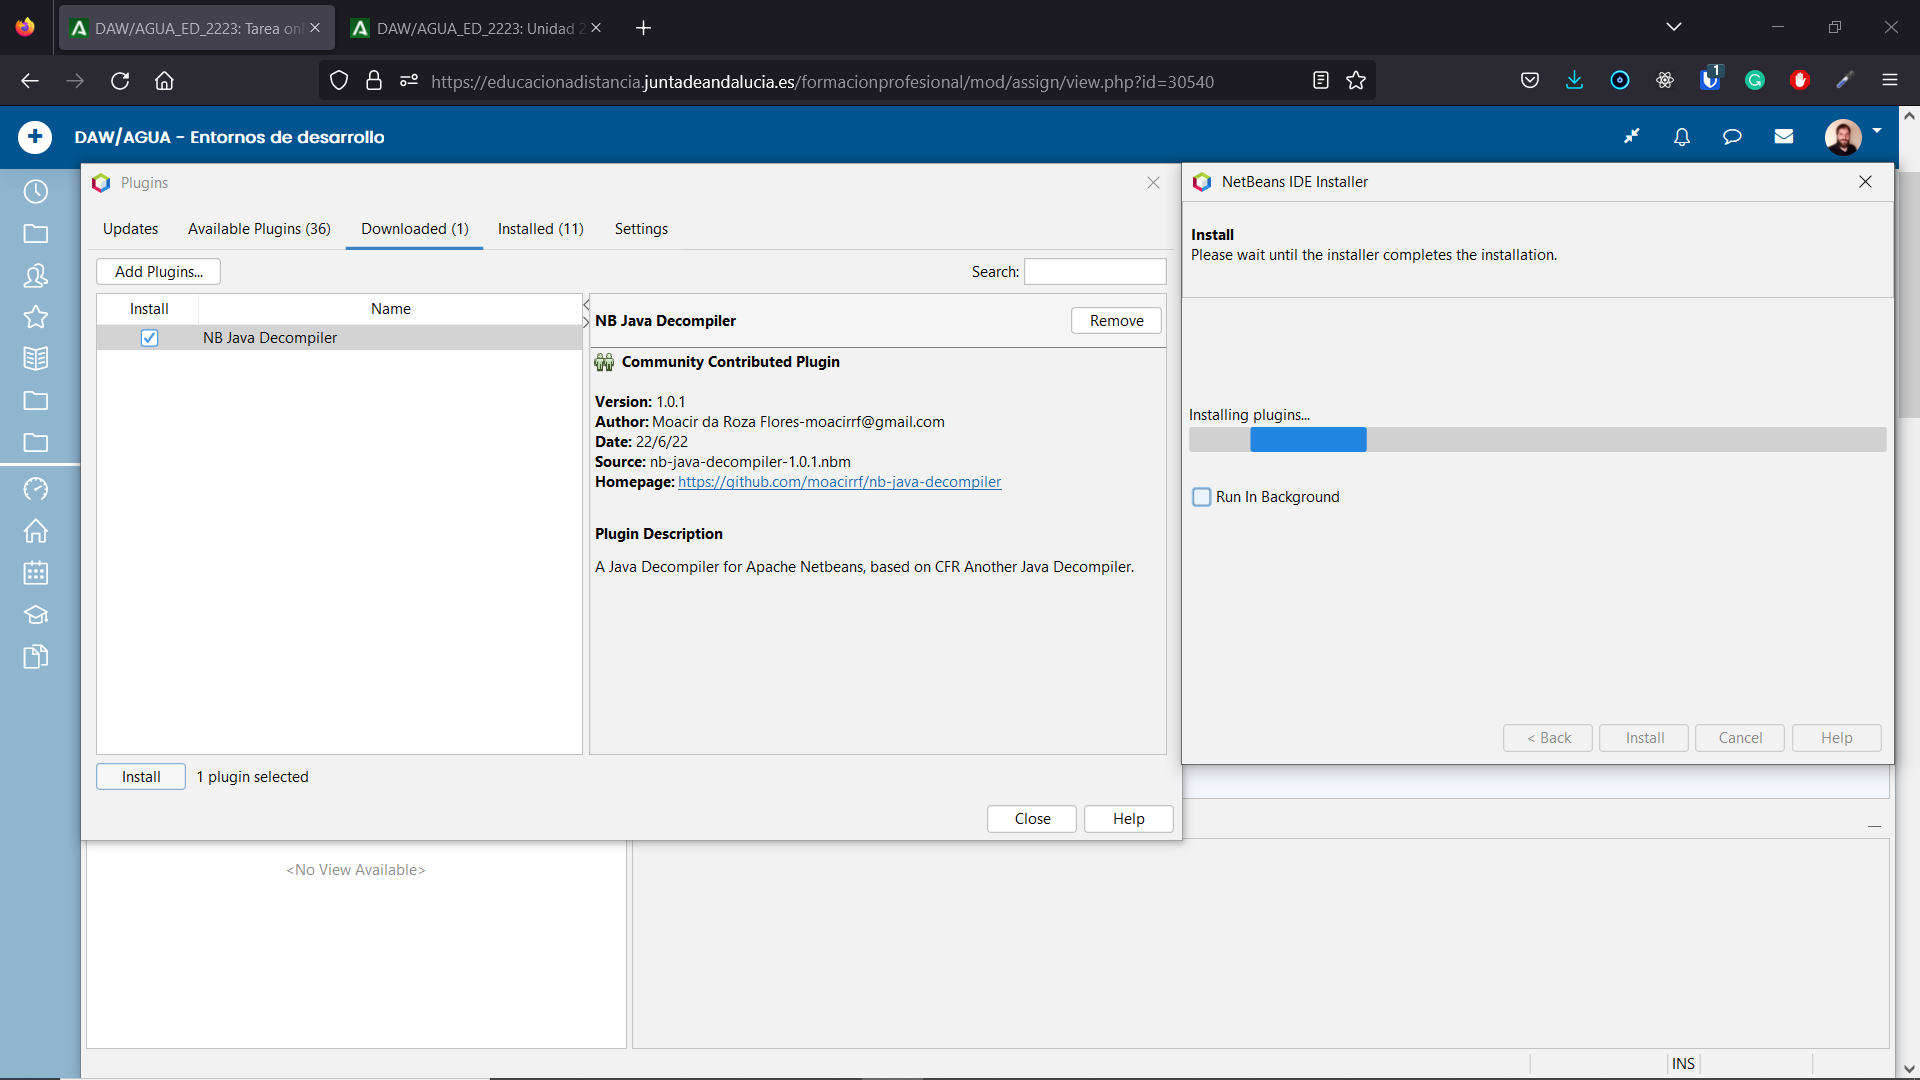
\includegraphics[scale=0.32]{netbeans-plugins-1.png}
        \caption{NB Java Decompile instalándose de forma off-line}
    \end{figure}

    \begin{figure}[H]
        \centering
        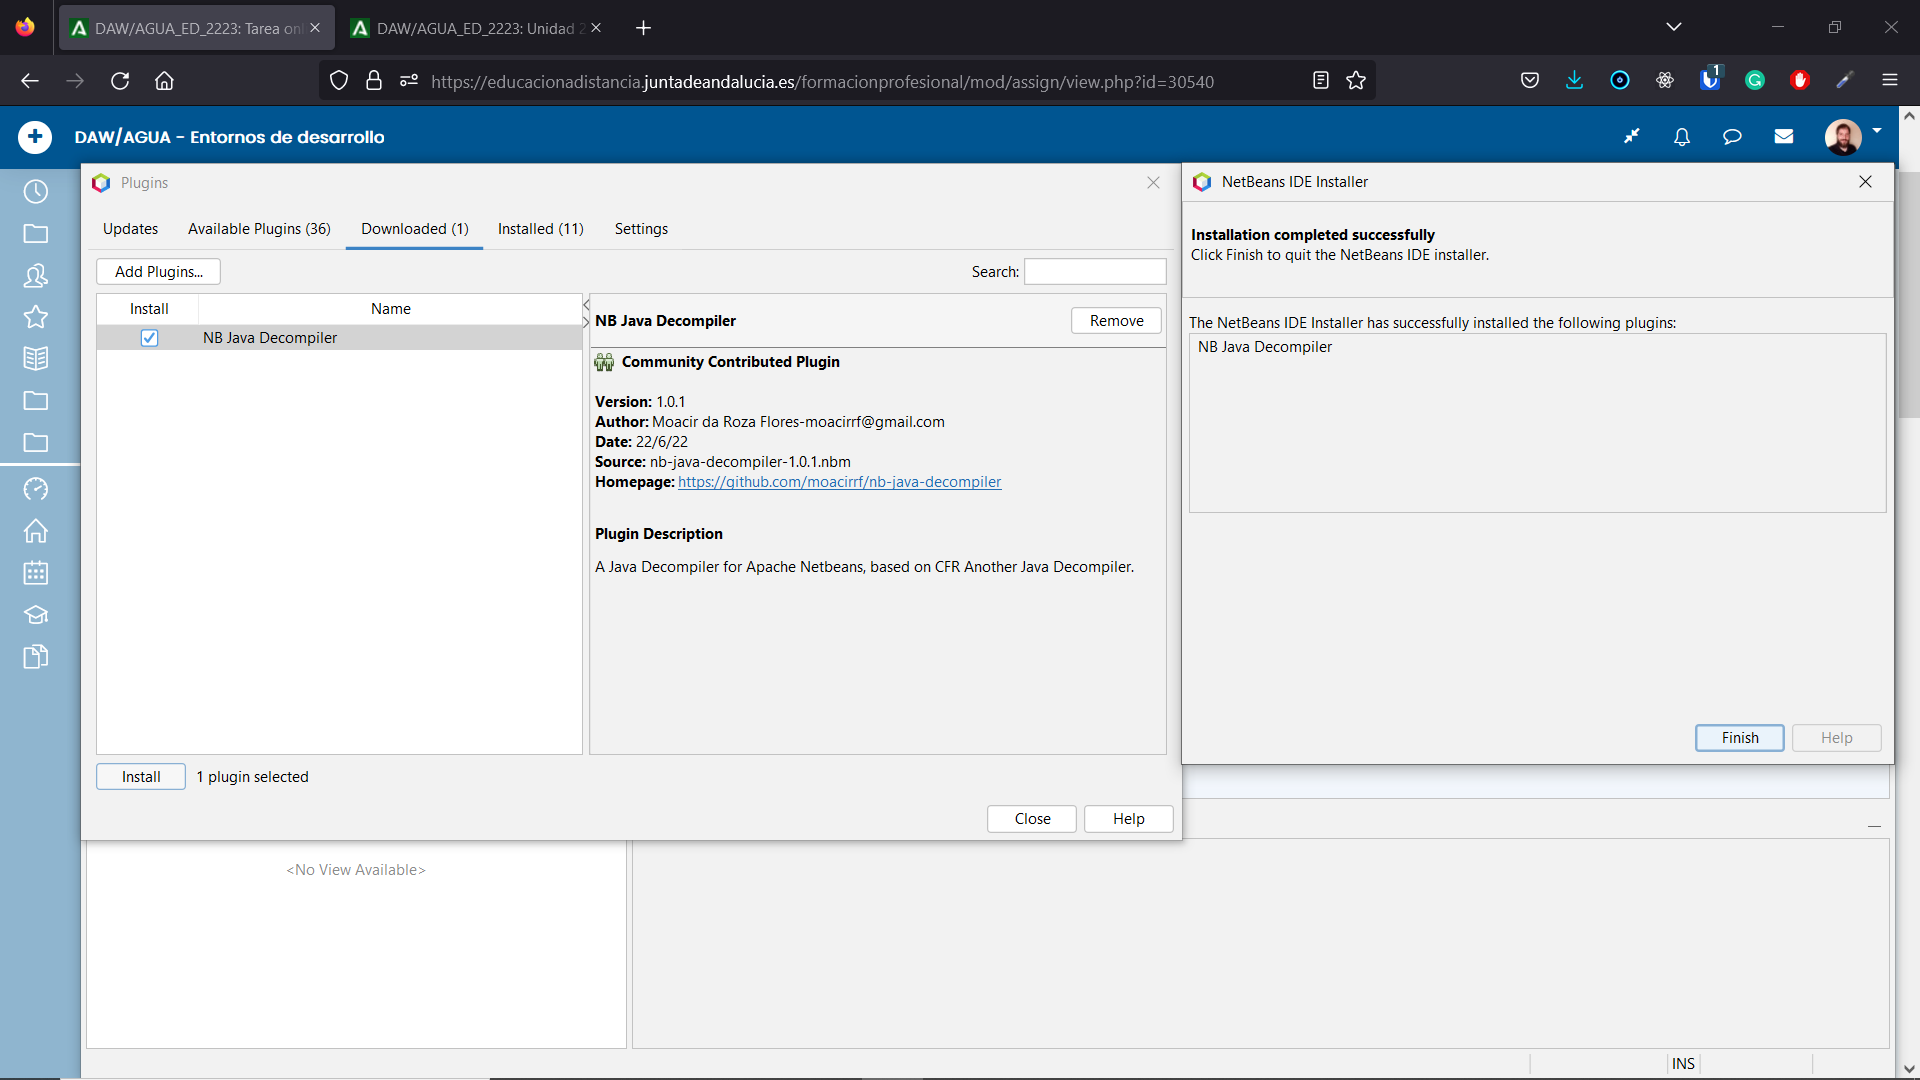
\includegraphics[scale=0.32]{netbeans-plugins-2.png}
        \caption{Instalación de NB Java Decompile completada}
    \end{figure}

    \item En segundo lugar instalaremos \textbf{Explorer Location OS} de forma on-line. En este caso, solo necesitamos acceder a la pestaña \textit{``Avaible Plugins}, en la pantalla de gestión de los plugins, buscarlo e instalarlo. Al igual que antes, puede aparecernos una ventana con un aviso sobre la firma del plugin, pero si los estamos descargando de los repositorios oficiales no deberemos preocuparnos.

     \begin{figure}[H]
        \centering
        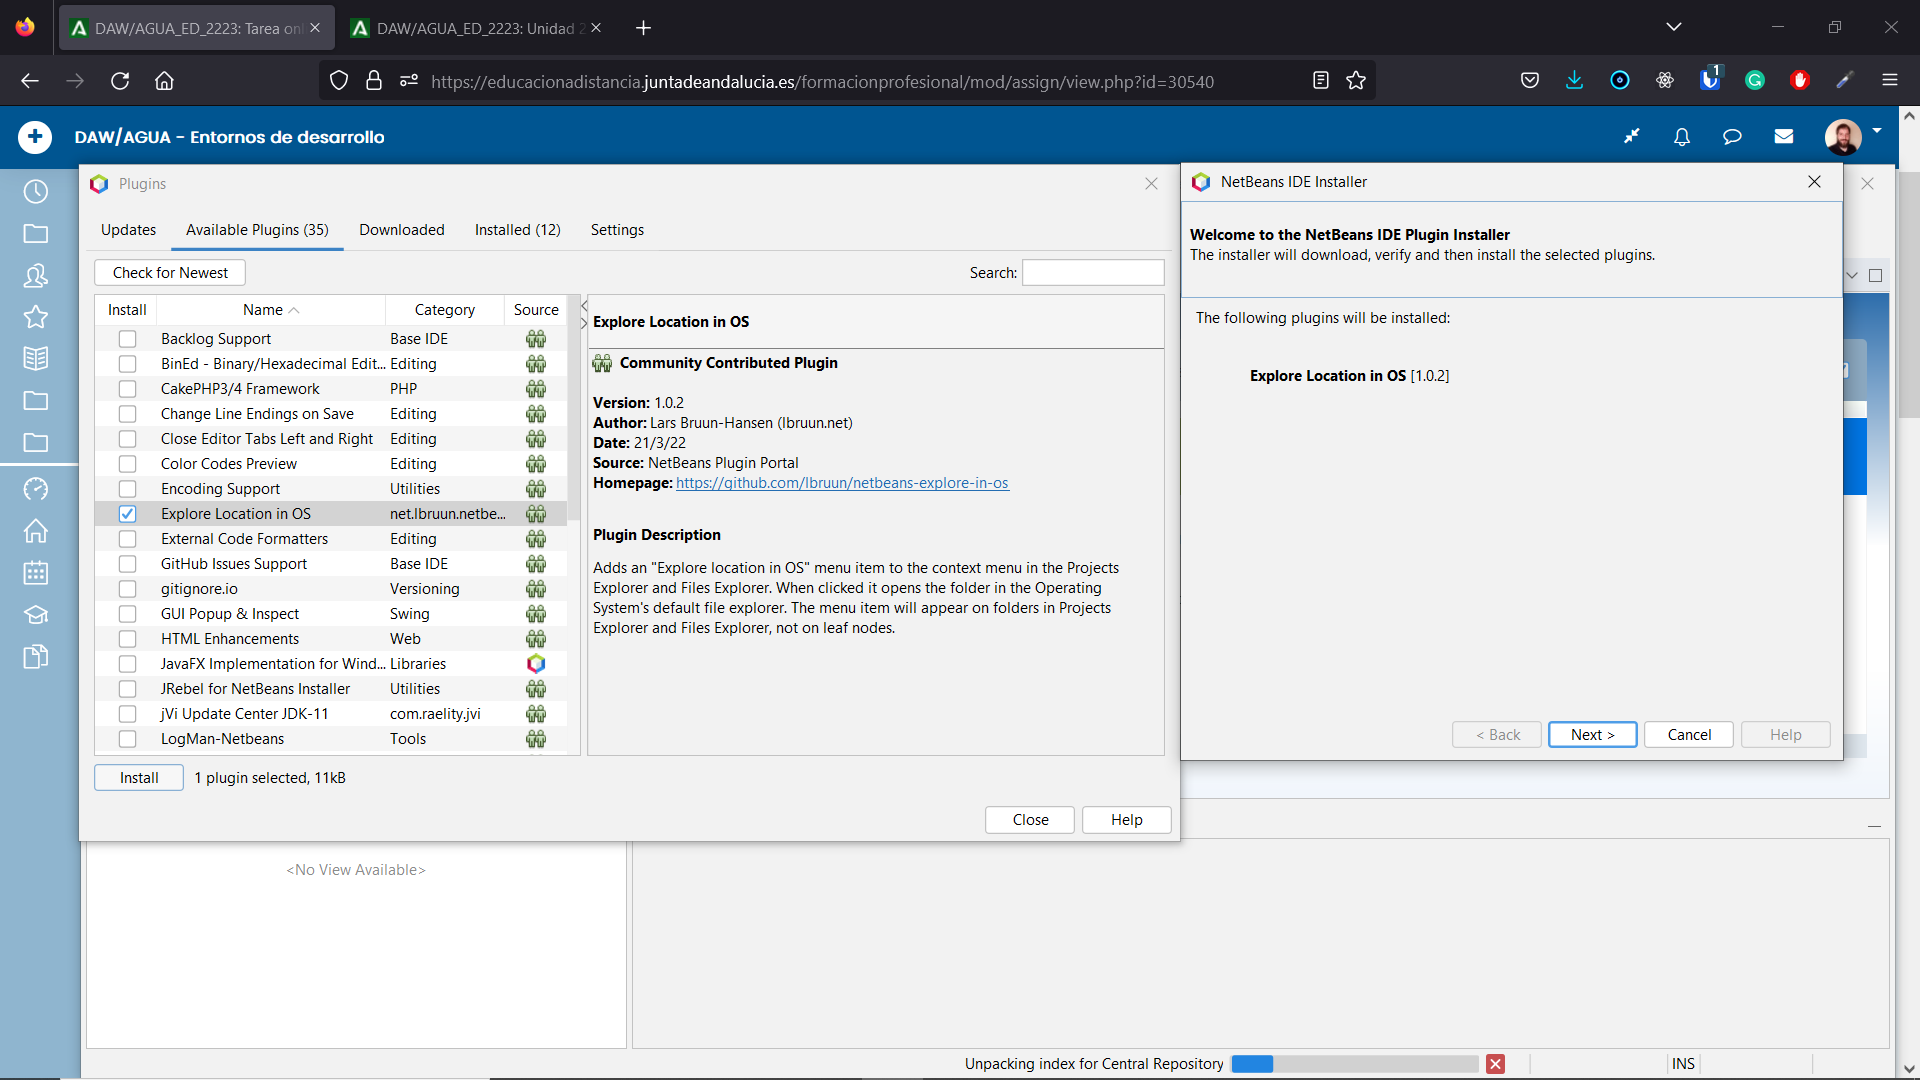
\includegraphics[scale=0.32]{netbeans-plugins-3.png}
        \caption{Explorer Location OS instalándose on-line}
    \end{figure}

    \begin{figure}[H]
        \centering
        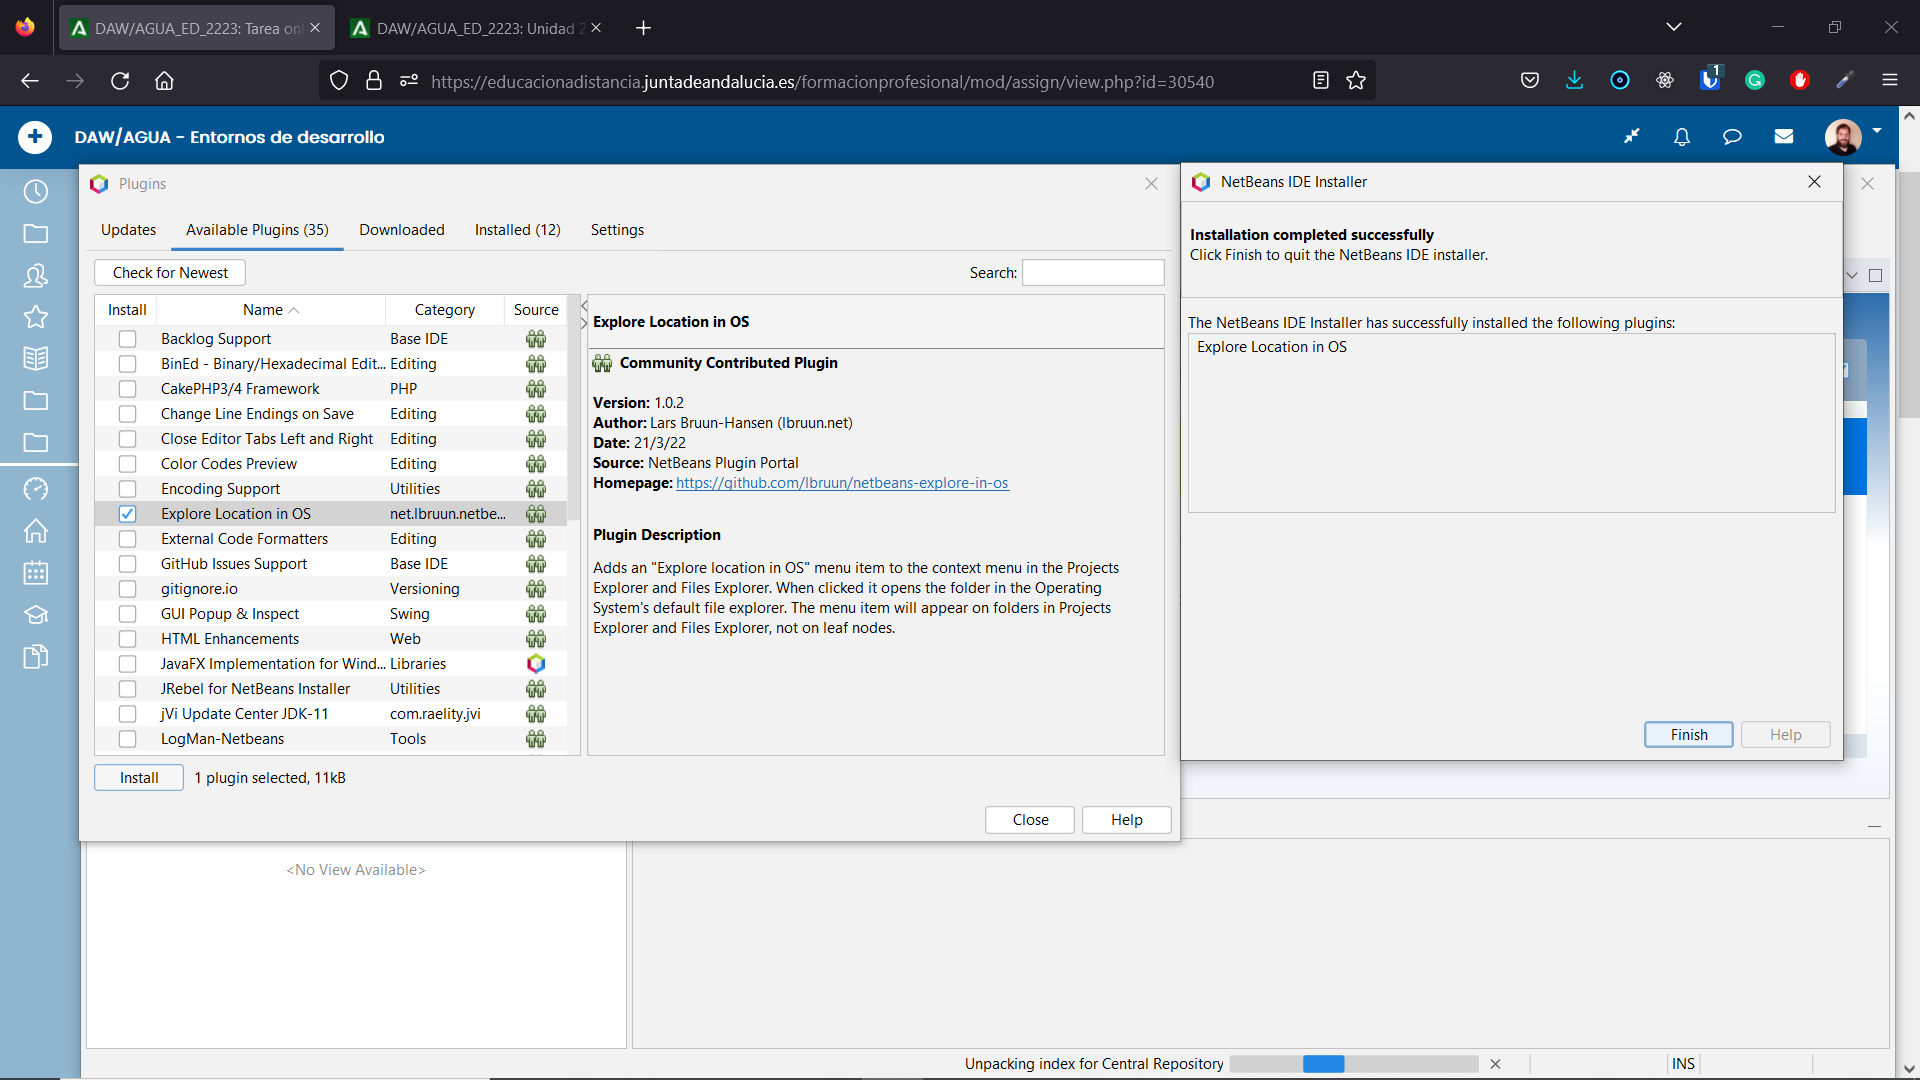
\includegraphics[scale=0.32]{netbeans-plugins-4.png}
        \caption{Instalación de NB Explorer Location OS completada}
    \end{figure}
\end{itemize}

\subsection{Actividad 4}
\subsubsection{Enunciado}
Actualiza el IDE y muestra la captura de pantalla de actualización o del mensaje de que no hay nada que actualizar.

Capturas solicitadas: 1

\subsubsection{Solución}
Ahora vamos a actualizar el IDE. Para ello, deberemos pulsar en el menú \textit{``Help''} y dentro de este en la opción \textit{``Check Updates''}. En el caso de que haya alguna actualización, se nos mostrará y podremos instalarla. En nuestro caso no había ninguna por lo que no ha sido necesario, como muestra la siguiente figura.

   \begin{figure}[H]
       \centering
        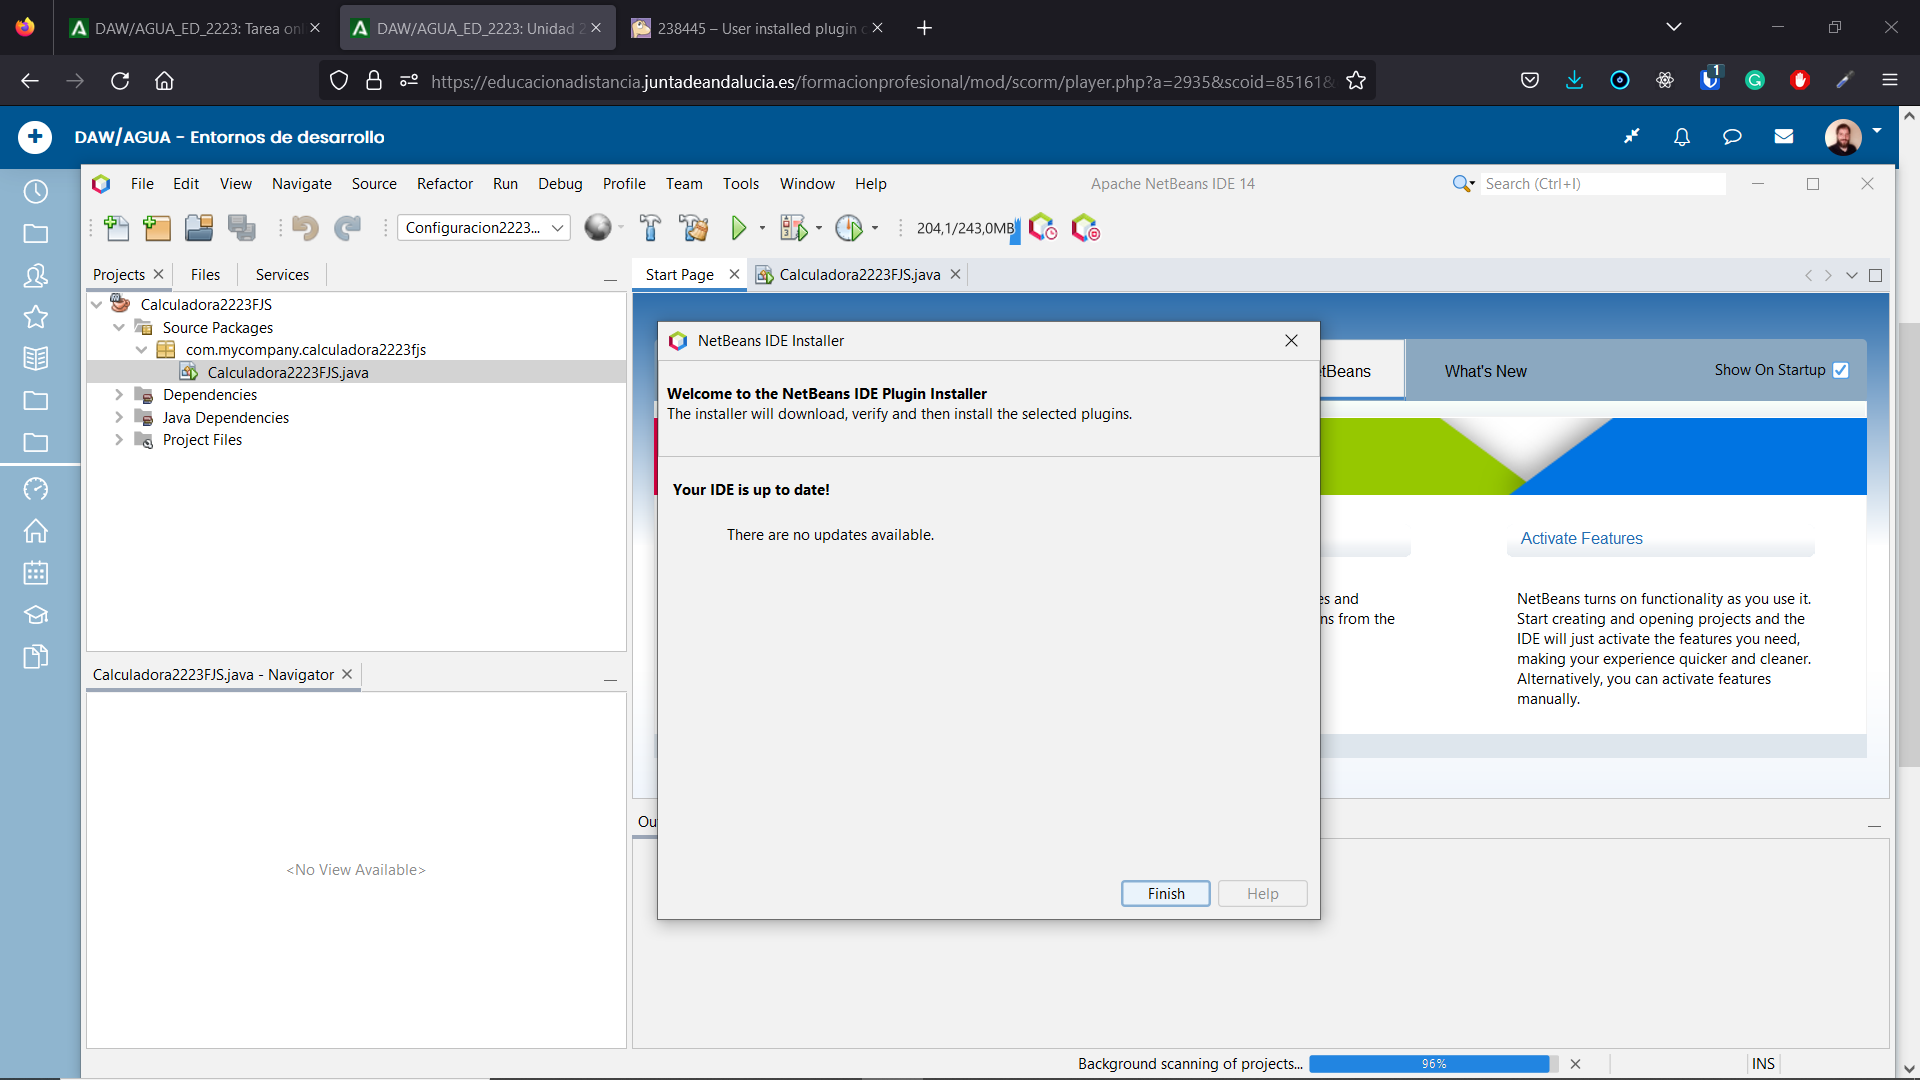
\includegraphics[scale=0.32]{netbeans-update.png}
        \caption{Pantalla de actualización de Netbeans}
    \end{figure}

\subsection{Actividad 5}
\subsubsection{Enunciado}
Desactiva el plugin Explore Location in OS y desintala el plugin NB Java Decompiler

Capturas solicitadas: 2
\begin{itemize}
    \item Captura de la ventana de plugins en la pestaña Installed, mostrando Explore Location in OS desactivado.
    \item Captura de la ventana de plugins en la pestaña Downloaded.
\end{itemize}

\subsubsection{Solución}
En esta actividad vamos a \textbf{desinstalar} uno de los plugins instalados en la actividad 3, en concreto vamos a desinstalar \textbf{NB Java Decompiler}, y vamos a \textbf{desactivar} el otro, \textbf{Explorer Location OS}.

Para llevar esto a cabo tenemos que pulsar en la pestaña \textit{``Installed''} de la ventana de gestión de plugins. Es probable, que de primeras no nos aparezcan, y en su lugar aparezcan los dos instalados bajo la opción \textbf{User Installed Plugins}. Si este fuera el caso, solo debemos marcar la casilla de la parte superior derecha llamada \textit{``Show Details''} y se nos mostrarán todos los plugins instalados de forma individual.

Una vez hecho esto, solo debemos desinstalar o deshabilitar el plugin que queramos. En caso de que el plugin desinstalado sea un plugin que hemos instalado de forma off-line volverá a aparecer en la pestaña \textit{``Downloaded''}, en caso de que lo hayamos instalado de forma on-line, podremos verlo deshabilitado en la misma pestaña \textit{``Installed''}. A continuación se muestran dos capturas con estas dos posibilidades.

\begin{figure}[H]
    \centering
    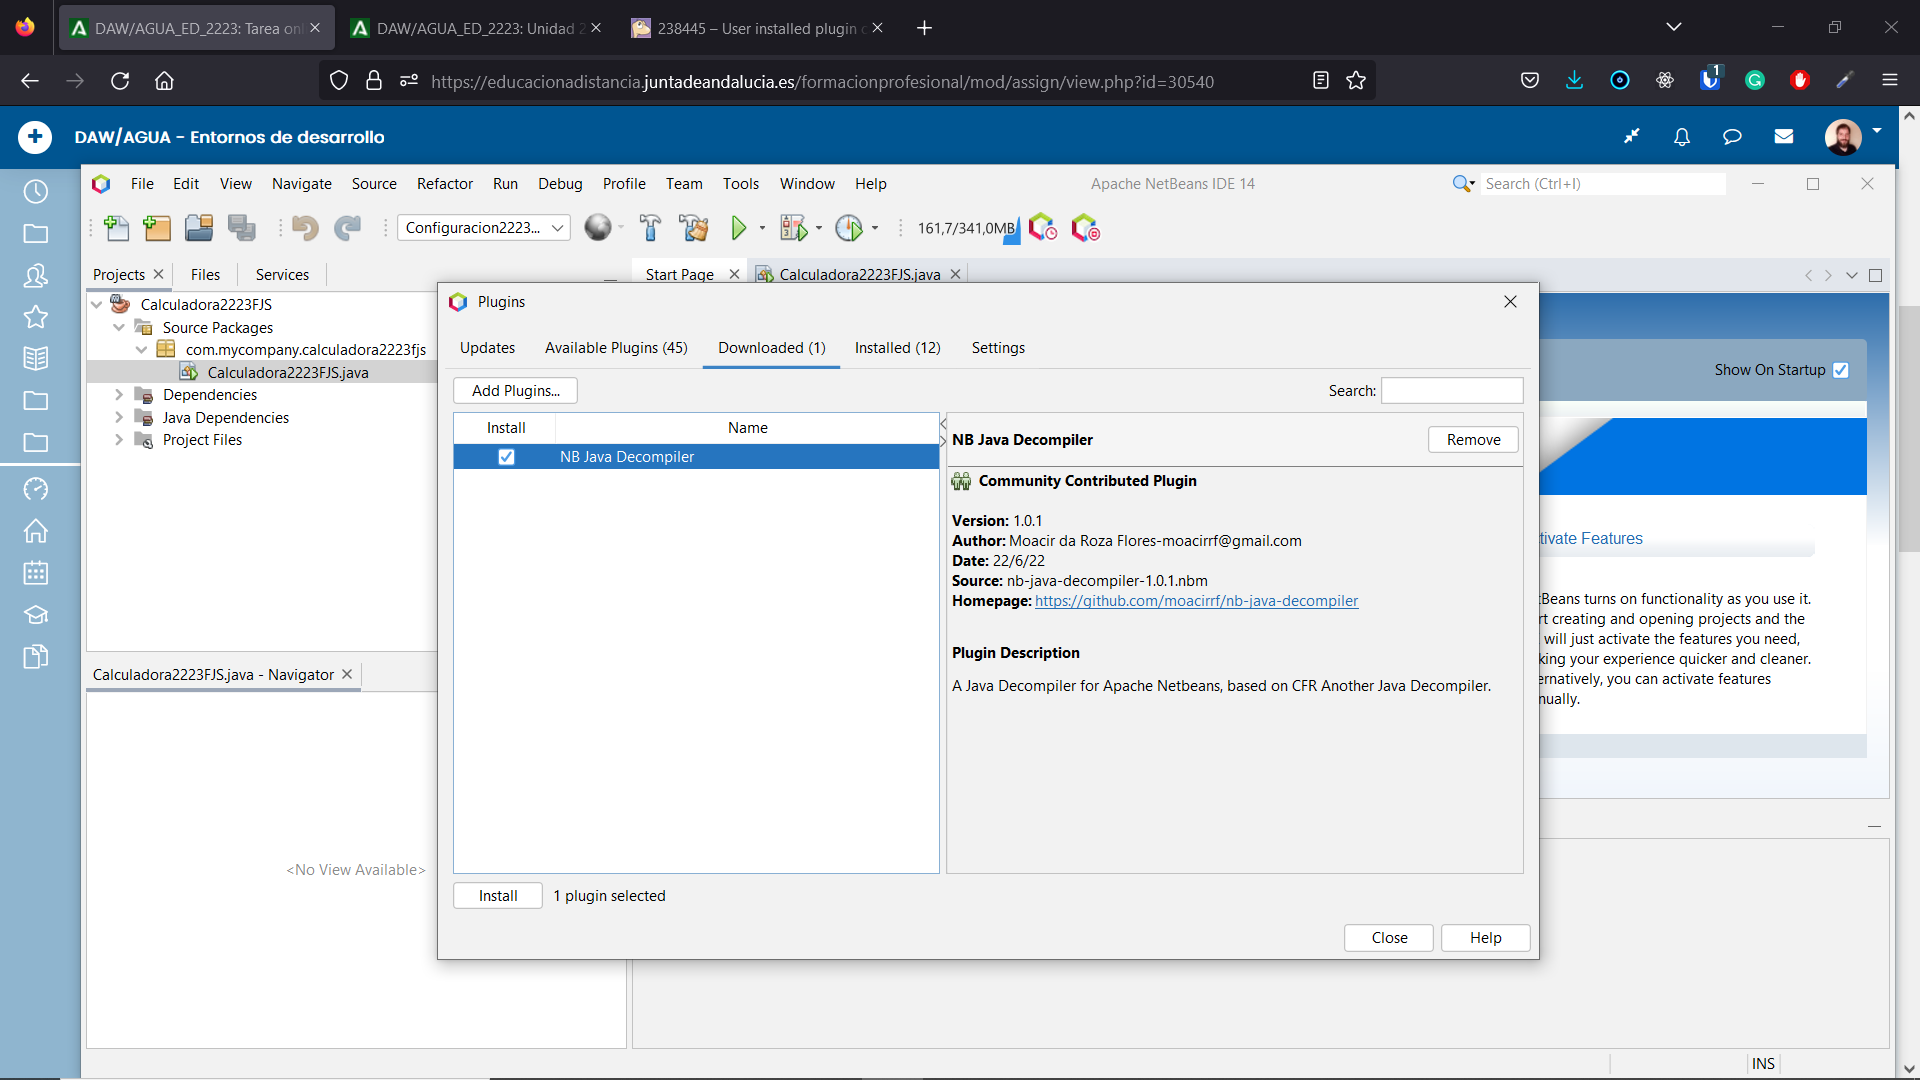
\includegraphics[scale=0.32]{netbeans-plugins-uninstall.png}
    \caption{Plugin NB Java Decompiler desinstalado}
\end{figure}

\begin{figure}[H]
    \centering
    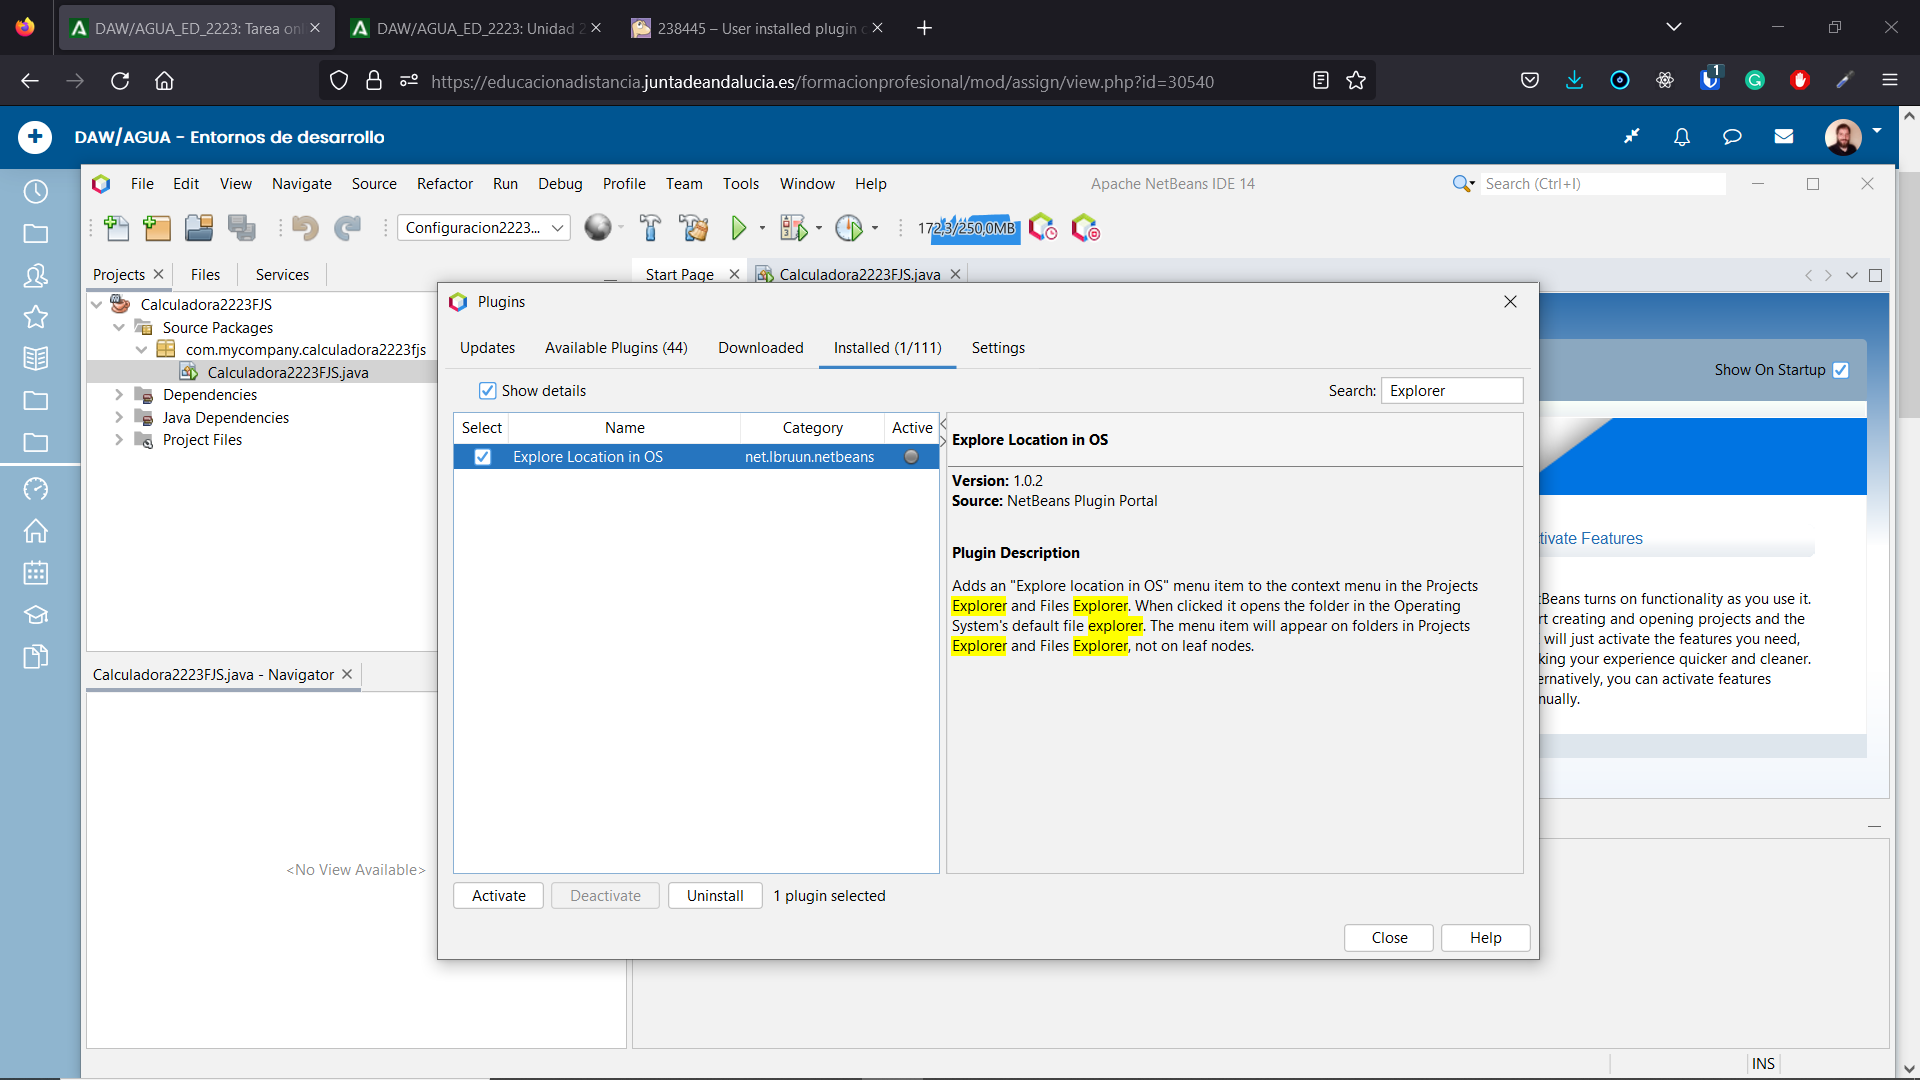
\includegraphics[scale=0.32]{netbeans-plugins-deactivate.png}
    \caption{Plugin Explorer Location in OS deshabilitado}
\end{figure}

\subsection{Actividad 6}
\subsubsection{Enunciado}
Escribe en la zona de edición de Netbeans el siguiente código Java:

\begin{itemize}
    \item \textbf{NOTA}: para que el código haya podido entrar en una misma página se han debido eliminar algunos comentarios y algunos espacios. Así mismo, las líneas más largas de código se han dividido en 2 líneas, en concreto algunas sentencias que incluyen System.out, aunque esto no debería causar ningún problema a la hora de copiar el código.
\end{itemize}

\begin{figure}[H]
    \begin{tcolorbox}[sharp corners, colback=yellow!30, colframe=white!20]
        \tiny
        \begin{verbatim}
package calculadora;

/** @author IES Aguadulce */

public class Calculadora {
    public static void main(String[] args) {
        int opcion = 0;

        Scanner sc;
        sc = new Scanner(System.in);
        int operando1, operando2;

        do{
            //Menú de consola
            System.out.println("\n");
            System.out.println("CALCULADORA DE NÚMEROS REALES:");
            System.out.println("1. Suma");
            System.out.println("2. Resta");
            System.out.println("3. Multiplicación");
            System.out.println("4. División");
            System.out.println("5. Resto");
            System.out.println("0. Salir");
            System.out.print("Introduzca una opción: ");

            opcion = Integer.parseInt(sc.nextLine());
            System.out.println();

            if (opcion>5 || opcion<0){
                System.out.println(Valor no válido. Introduzca un valor válido.);
            }
            else if (opcion = 0)
                System.out.println("Hasta pronto!!!"\n);

            else{
                System.out.print("Introduzca el primer operando: ");
                operando1 = Float.parseFloat(sc.nextLine());
                System.out.println();

                System.out.print("Introduzca el segundo operando: ");
                operando2 = Float.parseFloat(sc.nextLine());
                System.out.println();

                switch(opcion){
                    case 1:
                    System.out.println(
                    "La suma de  +operando1+ " y "+operando2 +" es " (operando1 + operando2));
                    break;
                    case 2:
                    System.out.println("La resta de " + operando1 + " y "+ operando2
                        + " es " (operando1 - operando2));
                    break;
                    case 3:
                    System.out.println("La multiplicación de  +operando1+  y "+operando2+" es "
                        + (operando1 * operando2));
                    break;
                    case 4:
                    System.out.println("La división de " +operando1+ " y "+operando2
                        +" es " (operando1 / operando2));
                    break;
                    case 5:
                    System.out.println("El resto de dividir " +operando1+ " y "+operando2
                        +" es "+ (operando1 % operando2));
                    break;
                }
            }
        }while(opcion == 0 || opcion != 0); //Si la opción es 0 sale del programa

        sc.close();//Indica que no vamos a volver a leer de teclado
        System.out.println("Ha finalizado el programa.");
    }
}         \end{verbatim}
    \end{tcolorbox}
    \caption{Código en Java para probar los IDEs}
\end{figure}

Siguiendo las indicaciones del editor corrige los fallos que indica y ejecuta el programa.

Capturas solicitadas: 2
\begin{itemize}
    \item Captura mostrando el proyecto con errores.
    \item Captura mostrando la salida de la ejecución.
\end{itemize}

\vspace{2ex}

\subsubsection{Solución}
Una vez creado el proyecto, hemos copiado el código que se nos propone en el enunciado, para una calculadora simple. Este código tiene diversos errores que impiden su ejecución, como se puede ver en la siguiente captura.

\begin{figure}[ht]
    \centering
    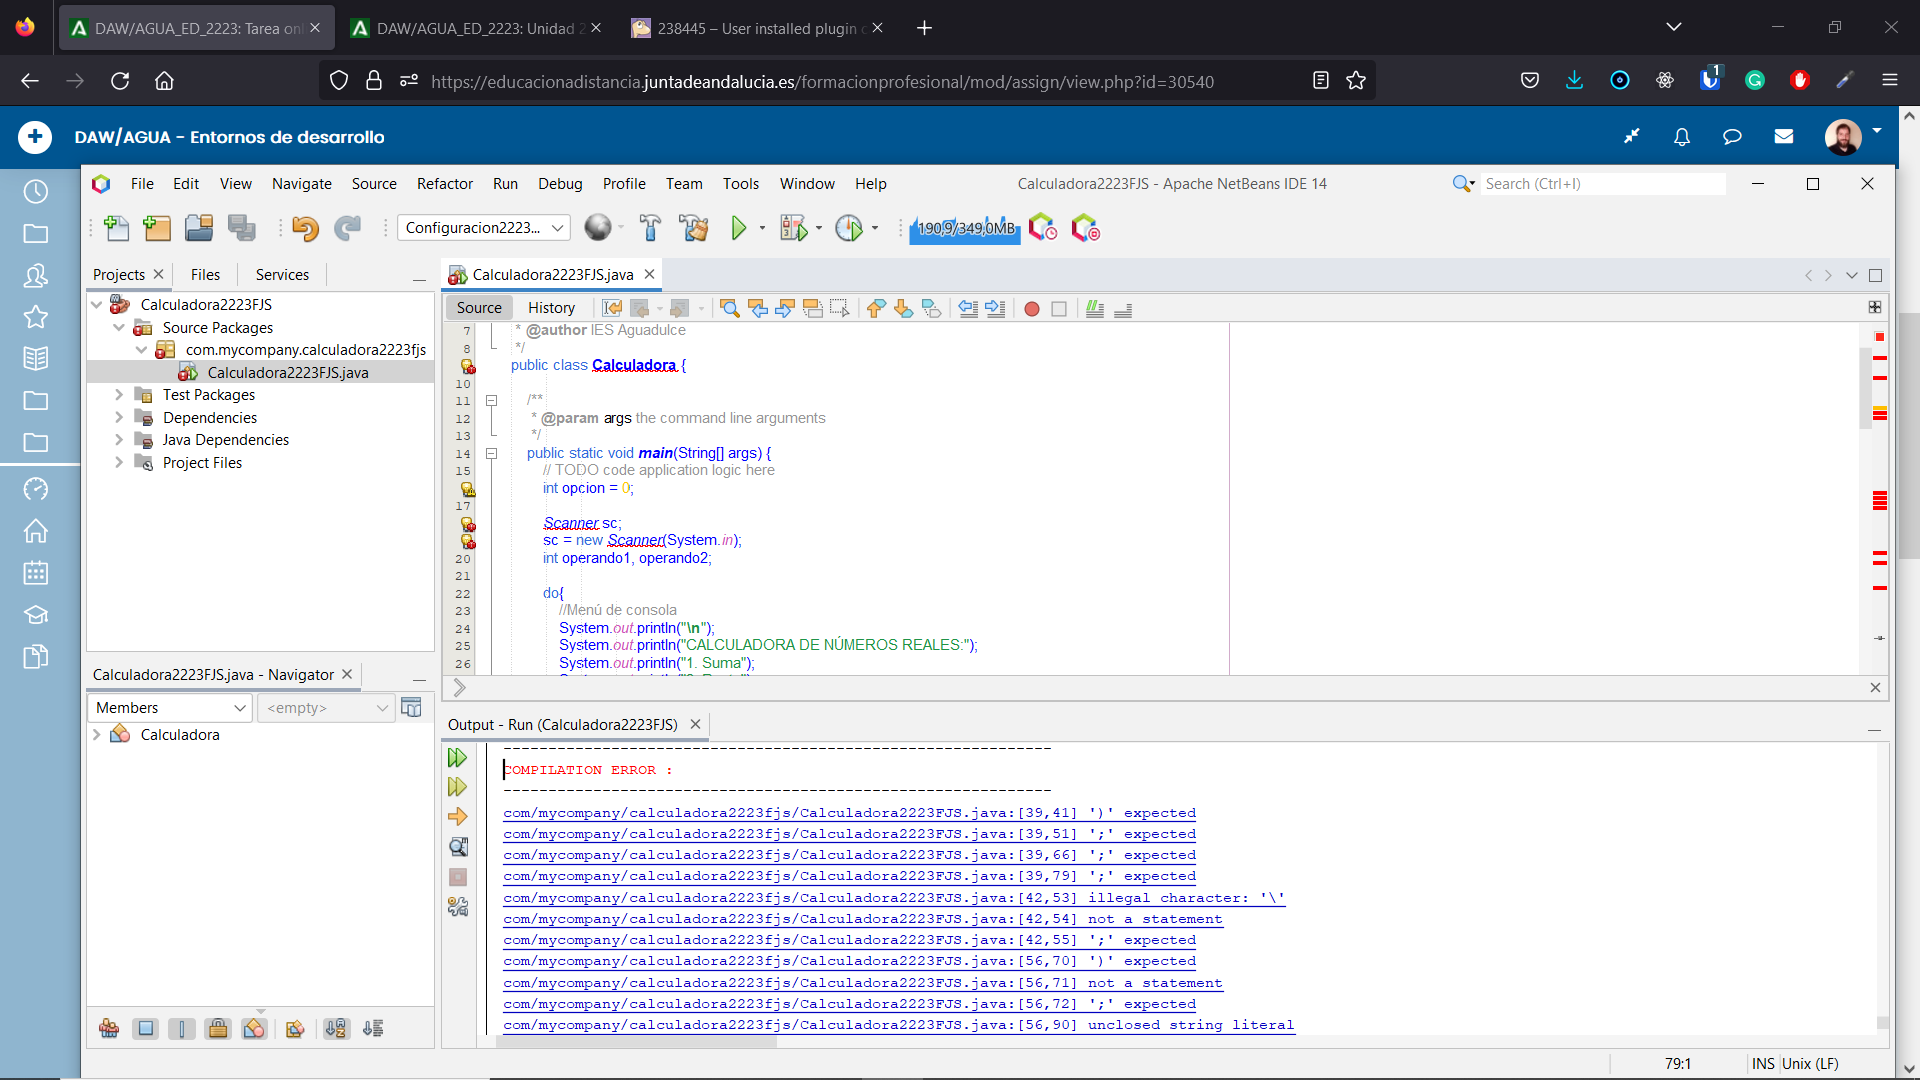
\includegraphics[scale=0.32]{netbeans-compilation-1.png}
    \caption{Código en Netbeans con errores}
\end{figure}

Una vez corregidos los diversos errores que tenía, entre ellos incompatibilidades de tipos, ausencia de algunos operadores en las cadenas de caracteres, etc.., se ha compilado de nuevo el código, pudiendo ejecutarse esta vez sin ningún problema.

\begin{figure}[ht]
    \centering
    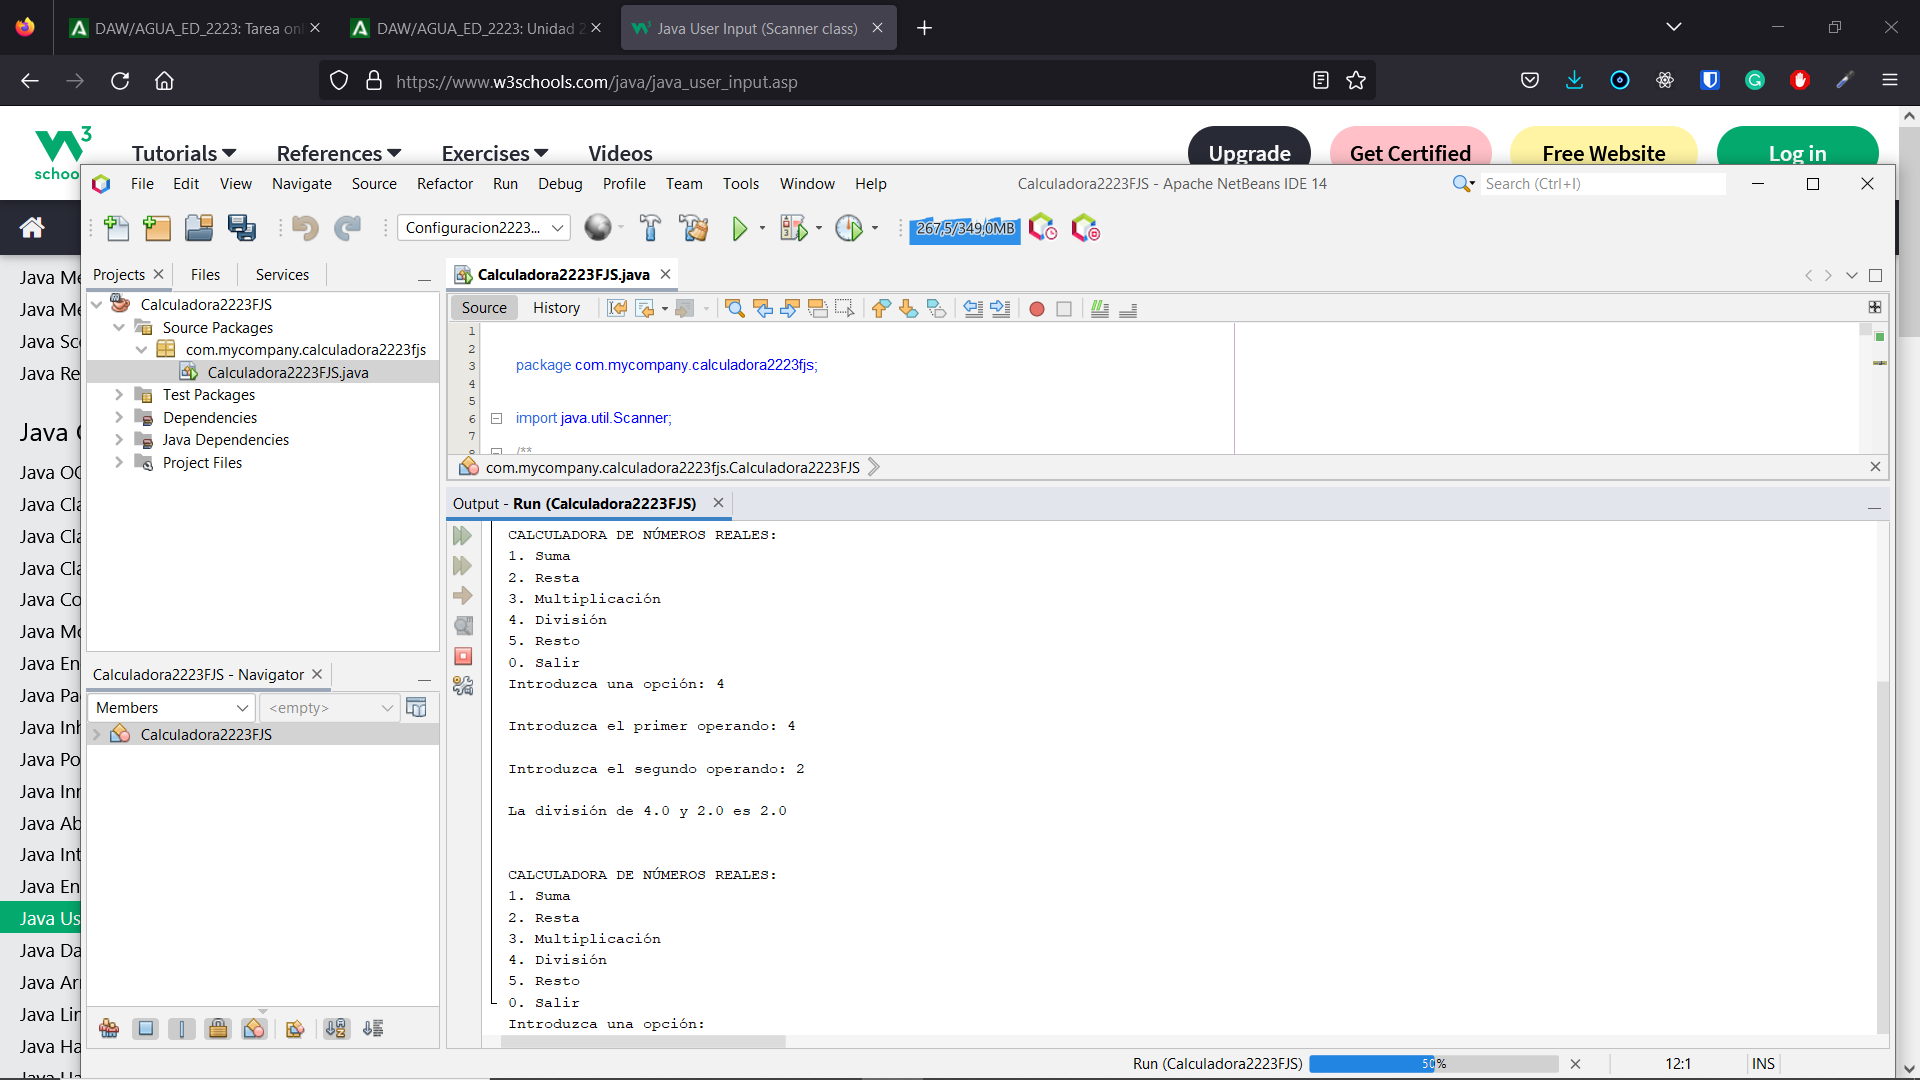
\includegraphics[scale=0.32]{netbeans-compilation-2.png}
    \caption{Código en Netbeans ejecutándose correctamente}
\end{figure}

\subsection{Actividad 7}
\subsubsection{Enunciado}
Descarga IntelliJ IDEA Community y realiza la instalación.

Capturas solicitadas: 2
\begin{itemize}
    \item Captura mostrando la versión que se va a instalar.
    \item Captura mostrando que el proceso de instalación ha finalizado correctamente.
\end{itemize}

\subsubsection{Solución}
En este ejercicio vamos a probar otro IDE diferente, en concreto, \textbf{IntelliJ IDEA} de \textbf{Jet Brains}.

Este IDE es uno de los más empleados en la actualidad para el desarrollo de aplicaciones en \textbf{Java} y \textbf{Kotlin}. Es un  IDE propietario y de pago, pero tiene una versión gratuita, la versión \textbf{Community}, la cual tiene menos prestaciones que la versión de pago pero es perfectamente funcional y nos sirve para desarrollar aplicaciones básicas de Java. \cite{intell01}

En el caso de que necesitemos algunas de las prestaciones que ofrece la versión de pago, como el soporte para Javascript o Reactjs, soporte de librerías como Spring, Jakarta EE o Java EE, así como algunas herramientas para bases de datos, podemos optar por la versión de pago, aunque todo hay que decirlo, no es especialmente económica, ya que el rango de precios oscila entre 59€ y 77€ al mes. \cite{intell02}

Nosotros hemos descargado la versión Community desde \href{https://www.jetbrains.com/idea/download/#section=windows}{la página oficial de Jet Brains}, y hemos comenzado su instalación.

\begin{figure}[ht]
    \centering
    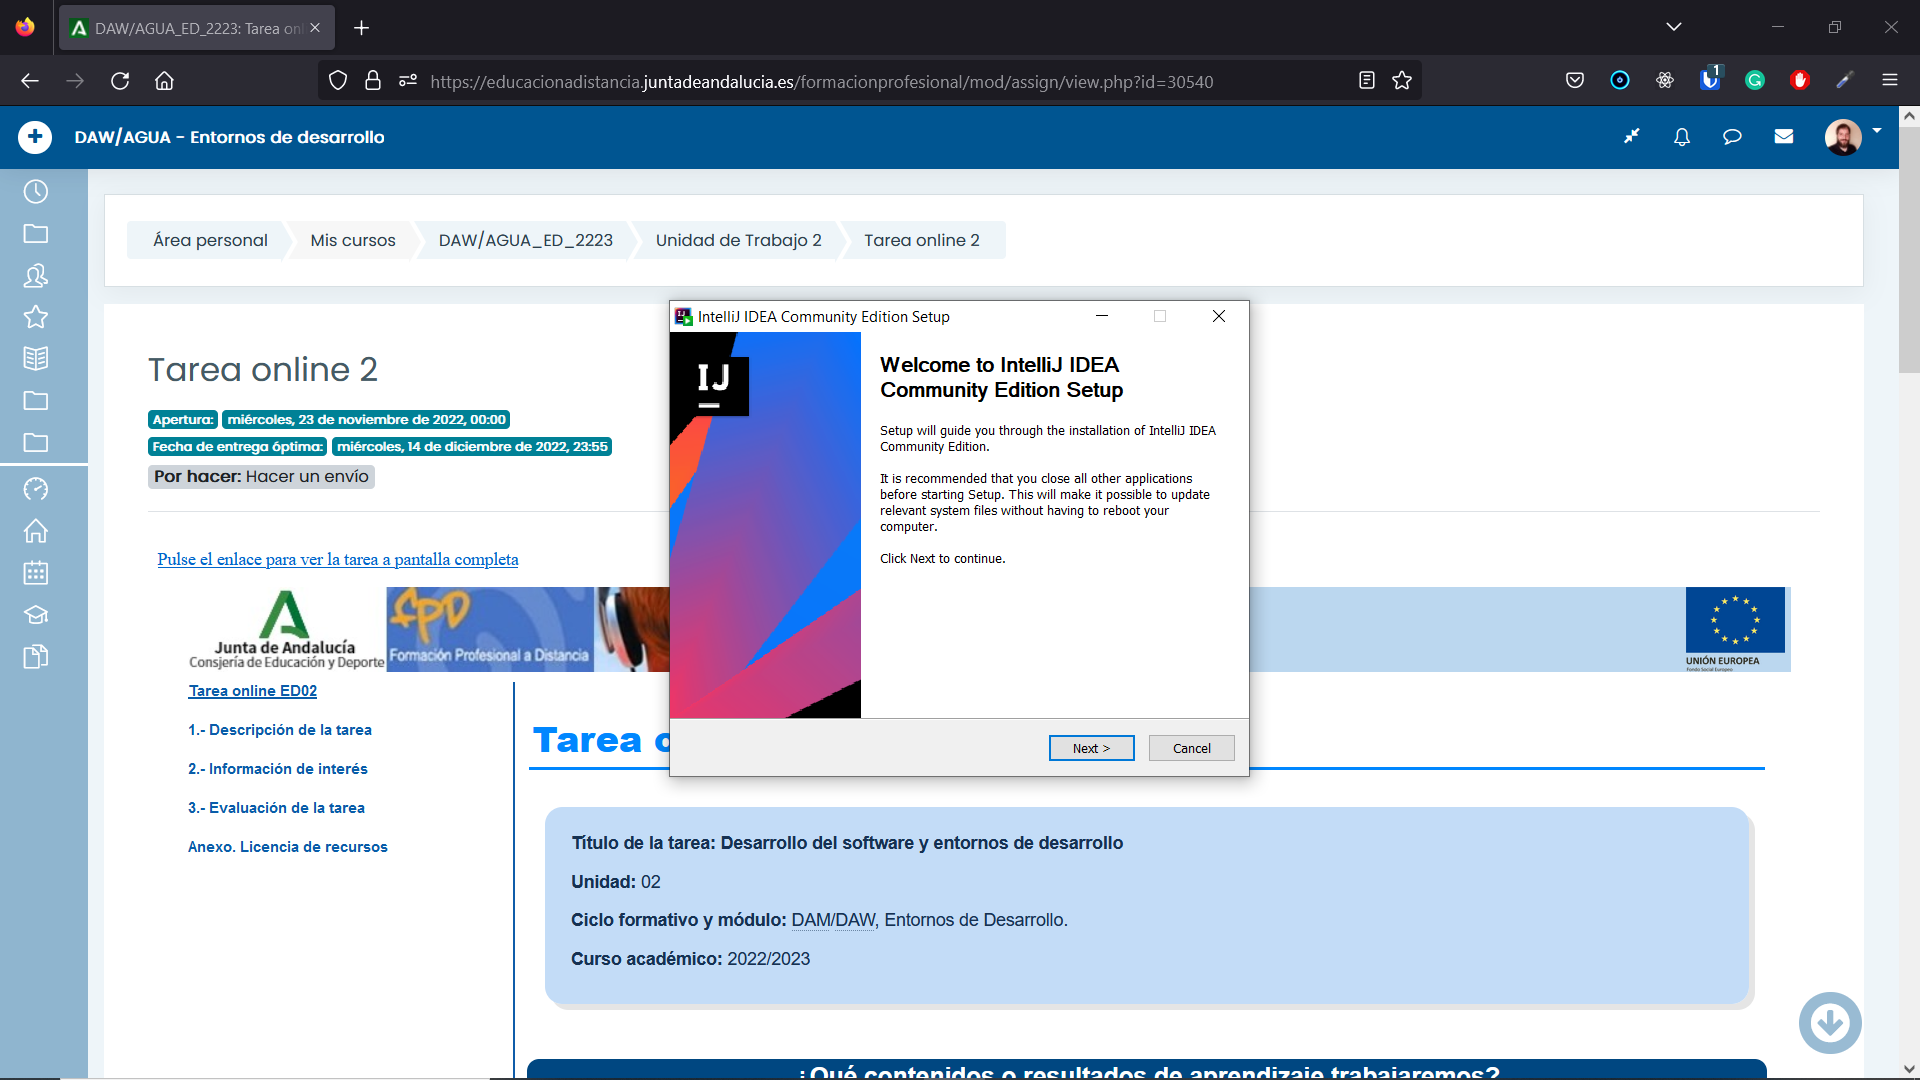
\includegraphics[scale=0.32]{idea-install-1.png}
    \caption{Inicio de instalación de IntelliJ versión Community}
\end{figure}

El proceso de instalación es simple, y nos pedirá algunas información durante el proceso por si queremos cambiar el directorio de instalación, pero podemos realizar la instalación con las opciones por defecto sin ningún problema. En la siguiente imagen vemos la que la instalación se ha realizado correctamente y que debemos reiniciar el ordenador.

\begin{figure}[ht]
    \centering
    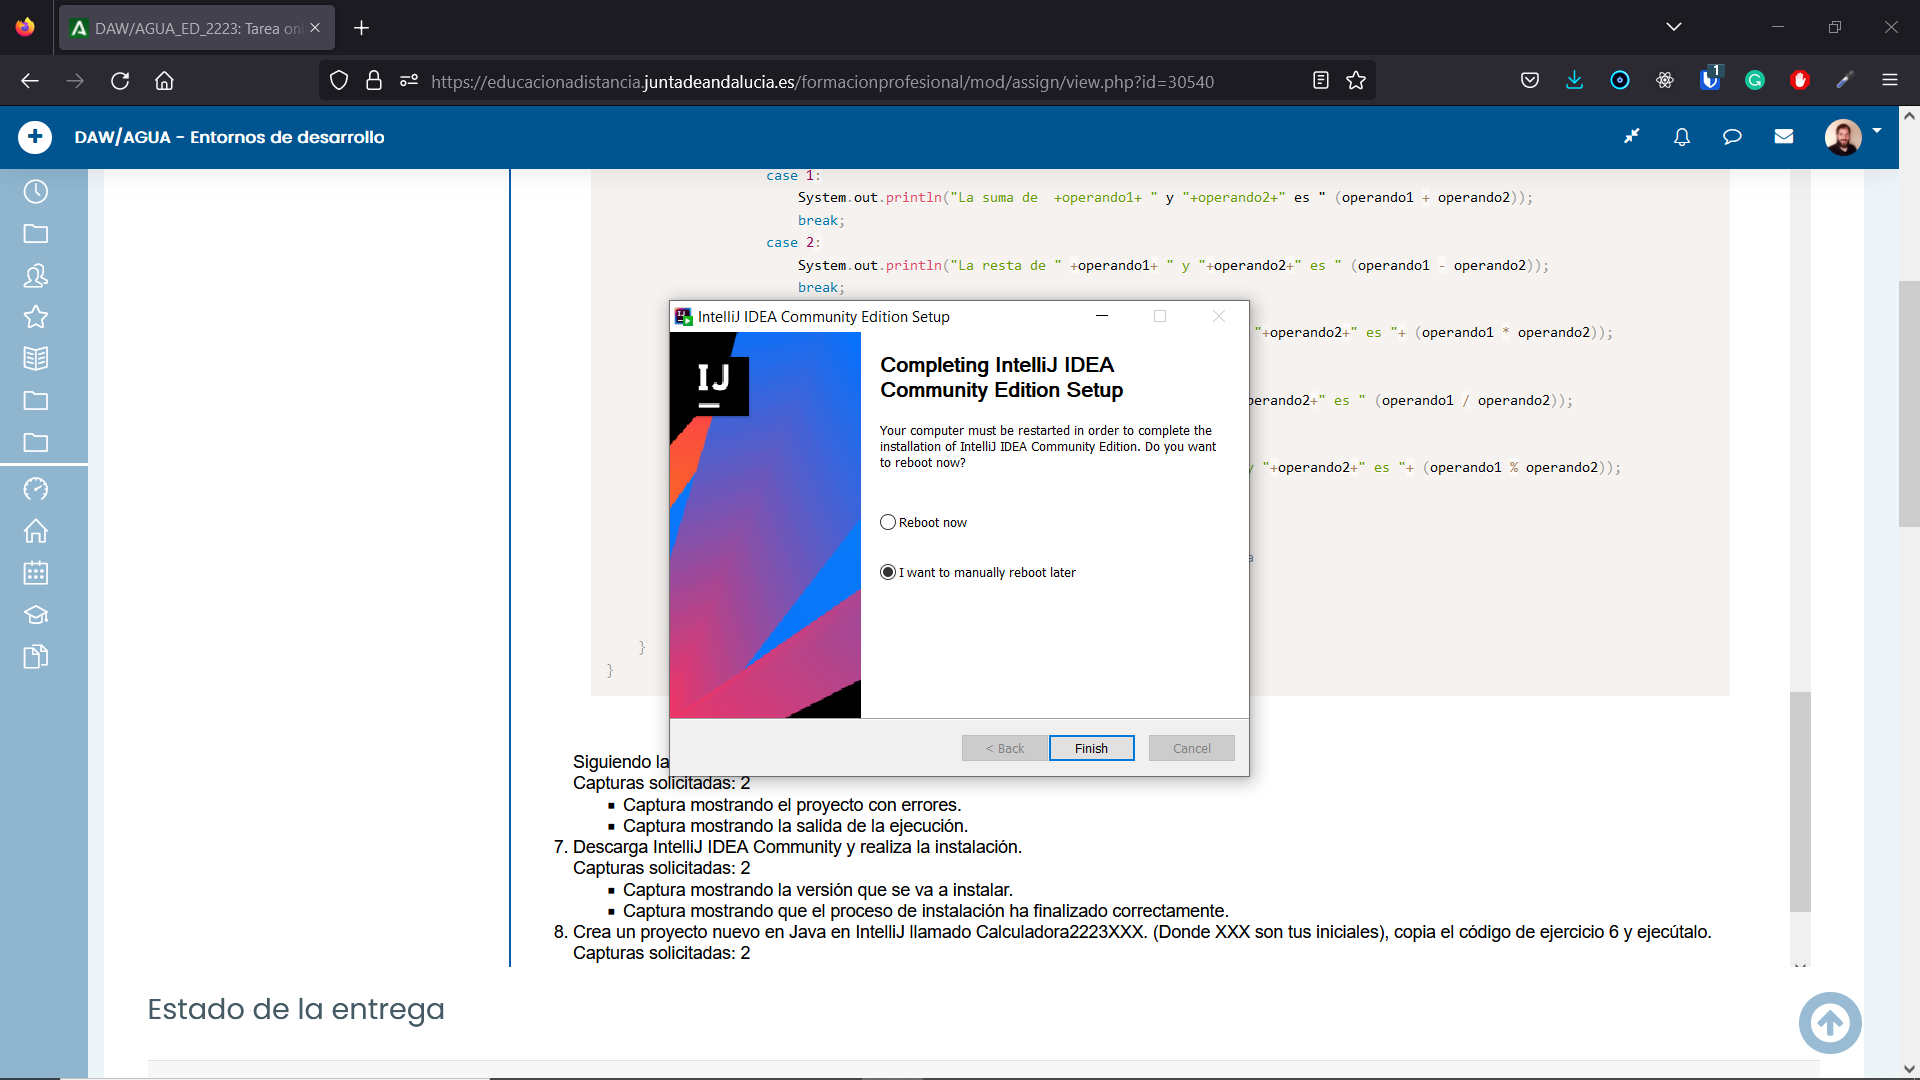
\includegraphics[scale=0.30]{idea-install-2.png}
    \caption{Instalación de Intellij IDEA completada}
\end{figure}

\subsection{Actividad 8}
\subsubsection{Enunciado}
Crea un proyecto nuevo en Java en IntelliJ llamado Calculadora2223XXX. (Donde XXX son tus iniciales), copia el código de ejercicio 6 y ejecútalo.

Capturas solicitadas: 2
\begin{itemize}
    \item Captura mostrando el proyecto.
    \item Captura mostrando la salida de la ejecución del programa.
\end{itemize}

\subsubsection{Solución}

En primer lugar hemos creado un proyecto con el nombre Calculadora2223FJS.

\begin{figure}[ht]
    \centering
    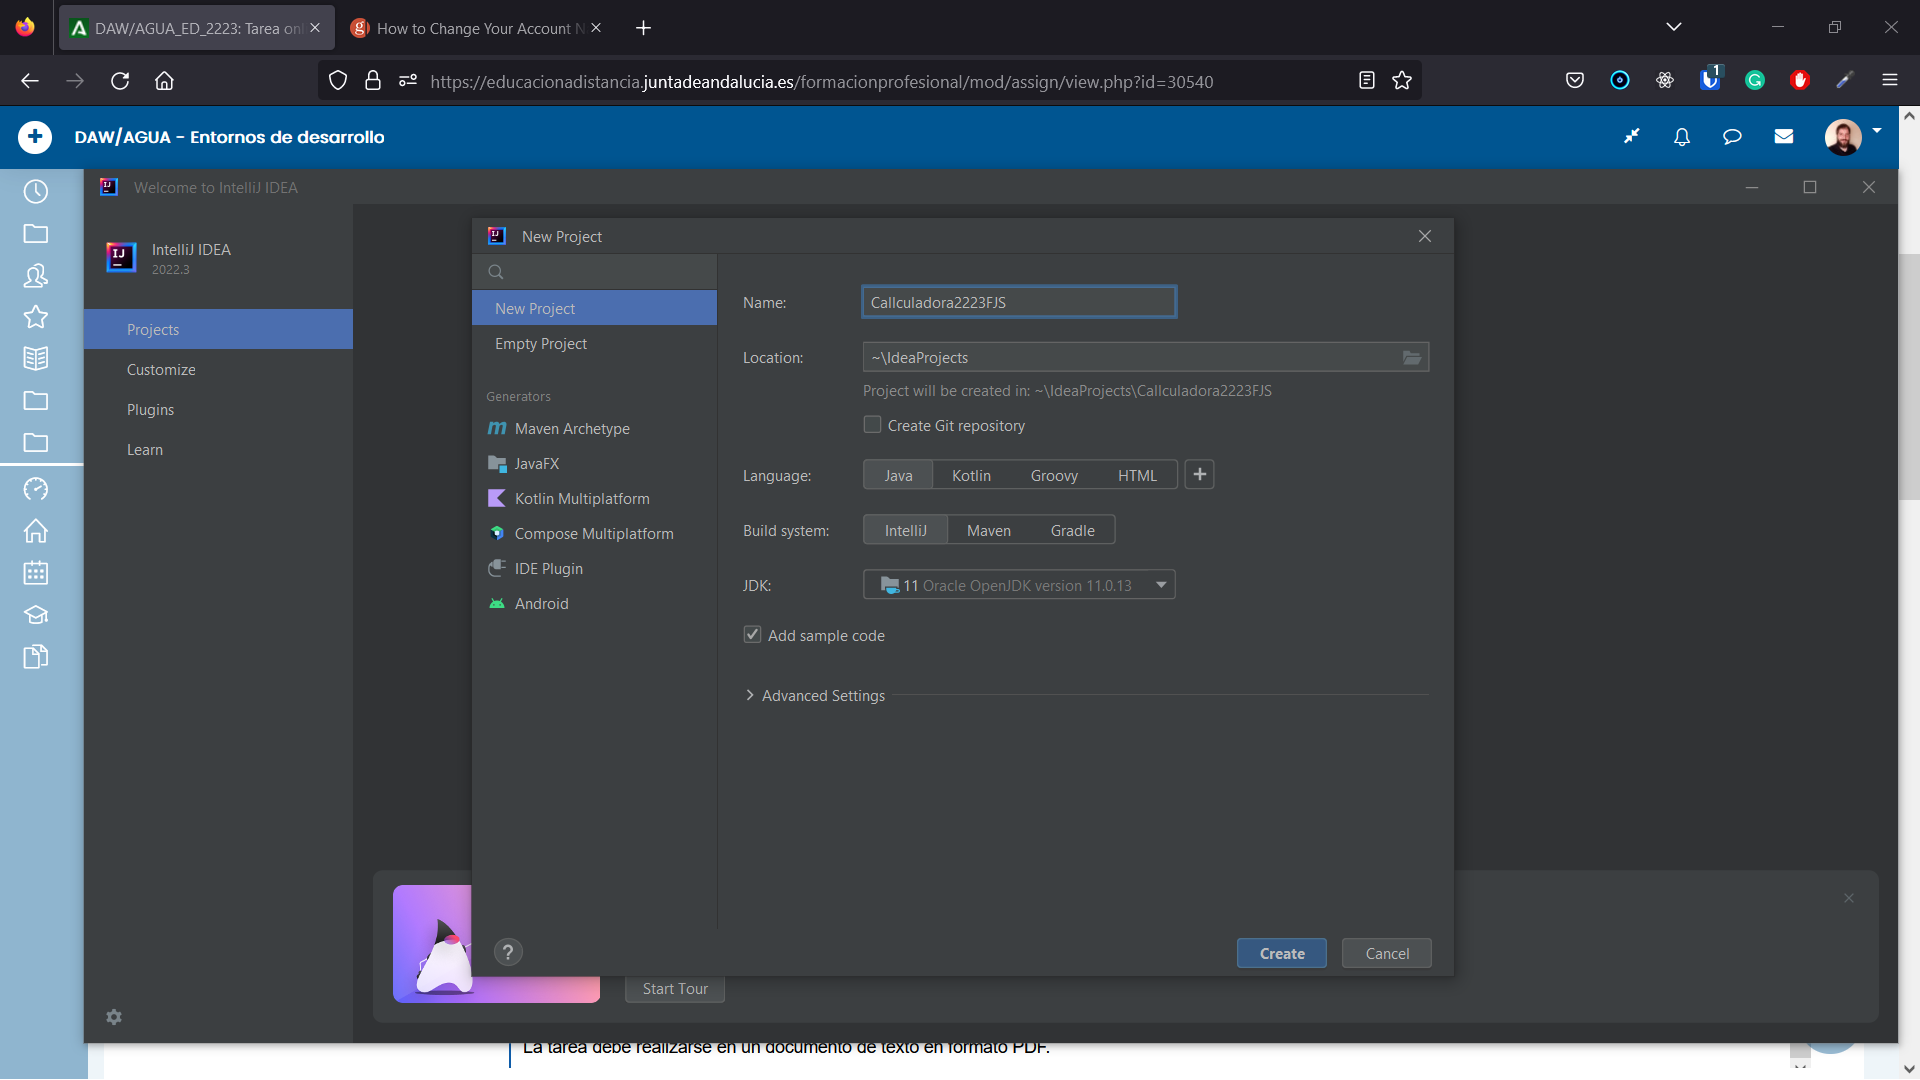
\includegraphics[scale=0.30]{idea-project.png}
    \caption{Creación del proyecto en IntelliJ}
\end{figure}

Una vez creado el proyecto se ha copiado el código de la calculadora que se especifica en el ejercicio 6. Como no nos ha quedado claro si el código que se debe copiar es el que tiene errores o se tiene que copiar el código ya corregido se han realizado capturas de los dos.

\begin{figure}[ht]
    \centering
    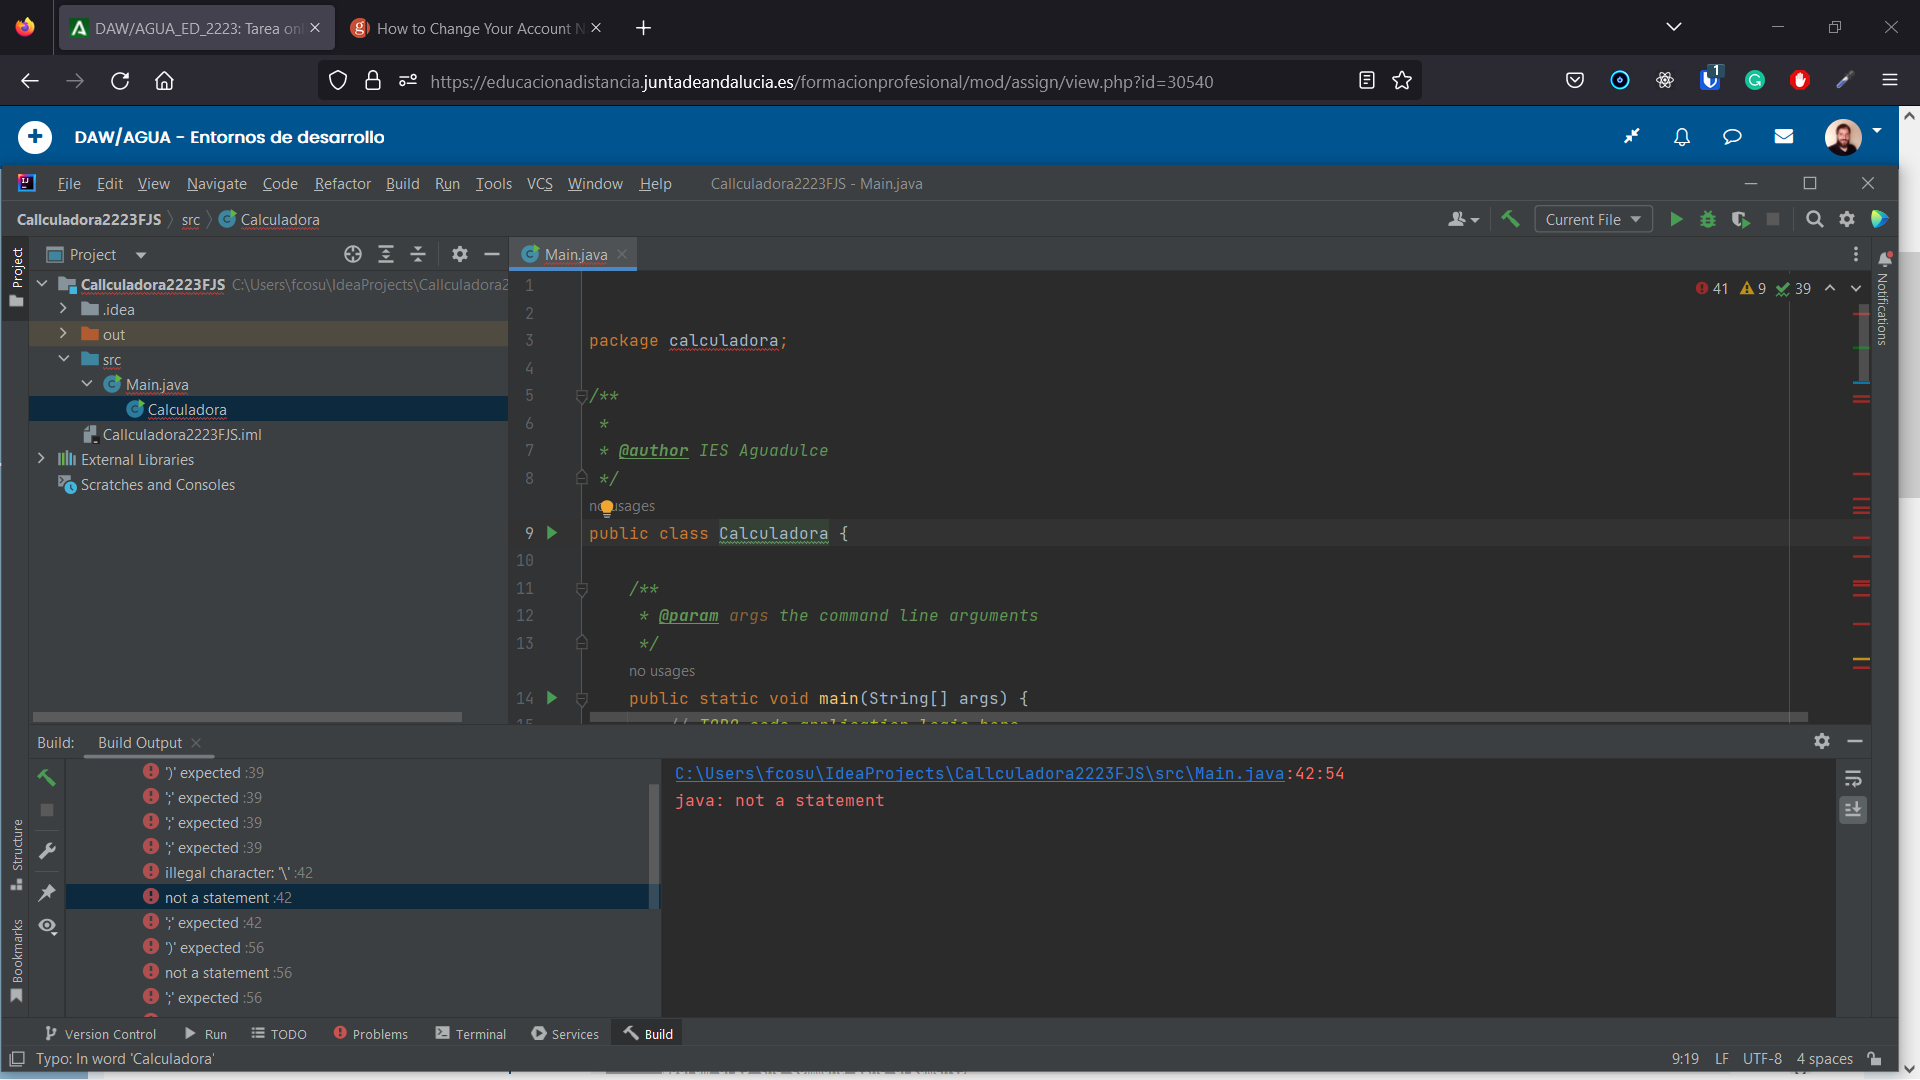
\includegraphics[scale=0.32]{idea-code-1.png}
    \caption{Código en IntelliJ con errores}
\end{figure}

\begin{figure}[ht]
    \centering
    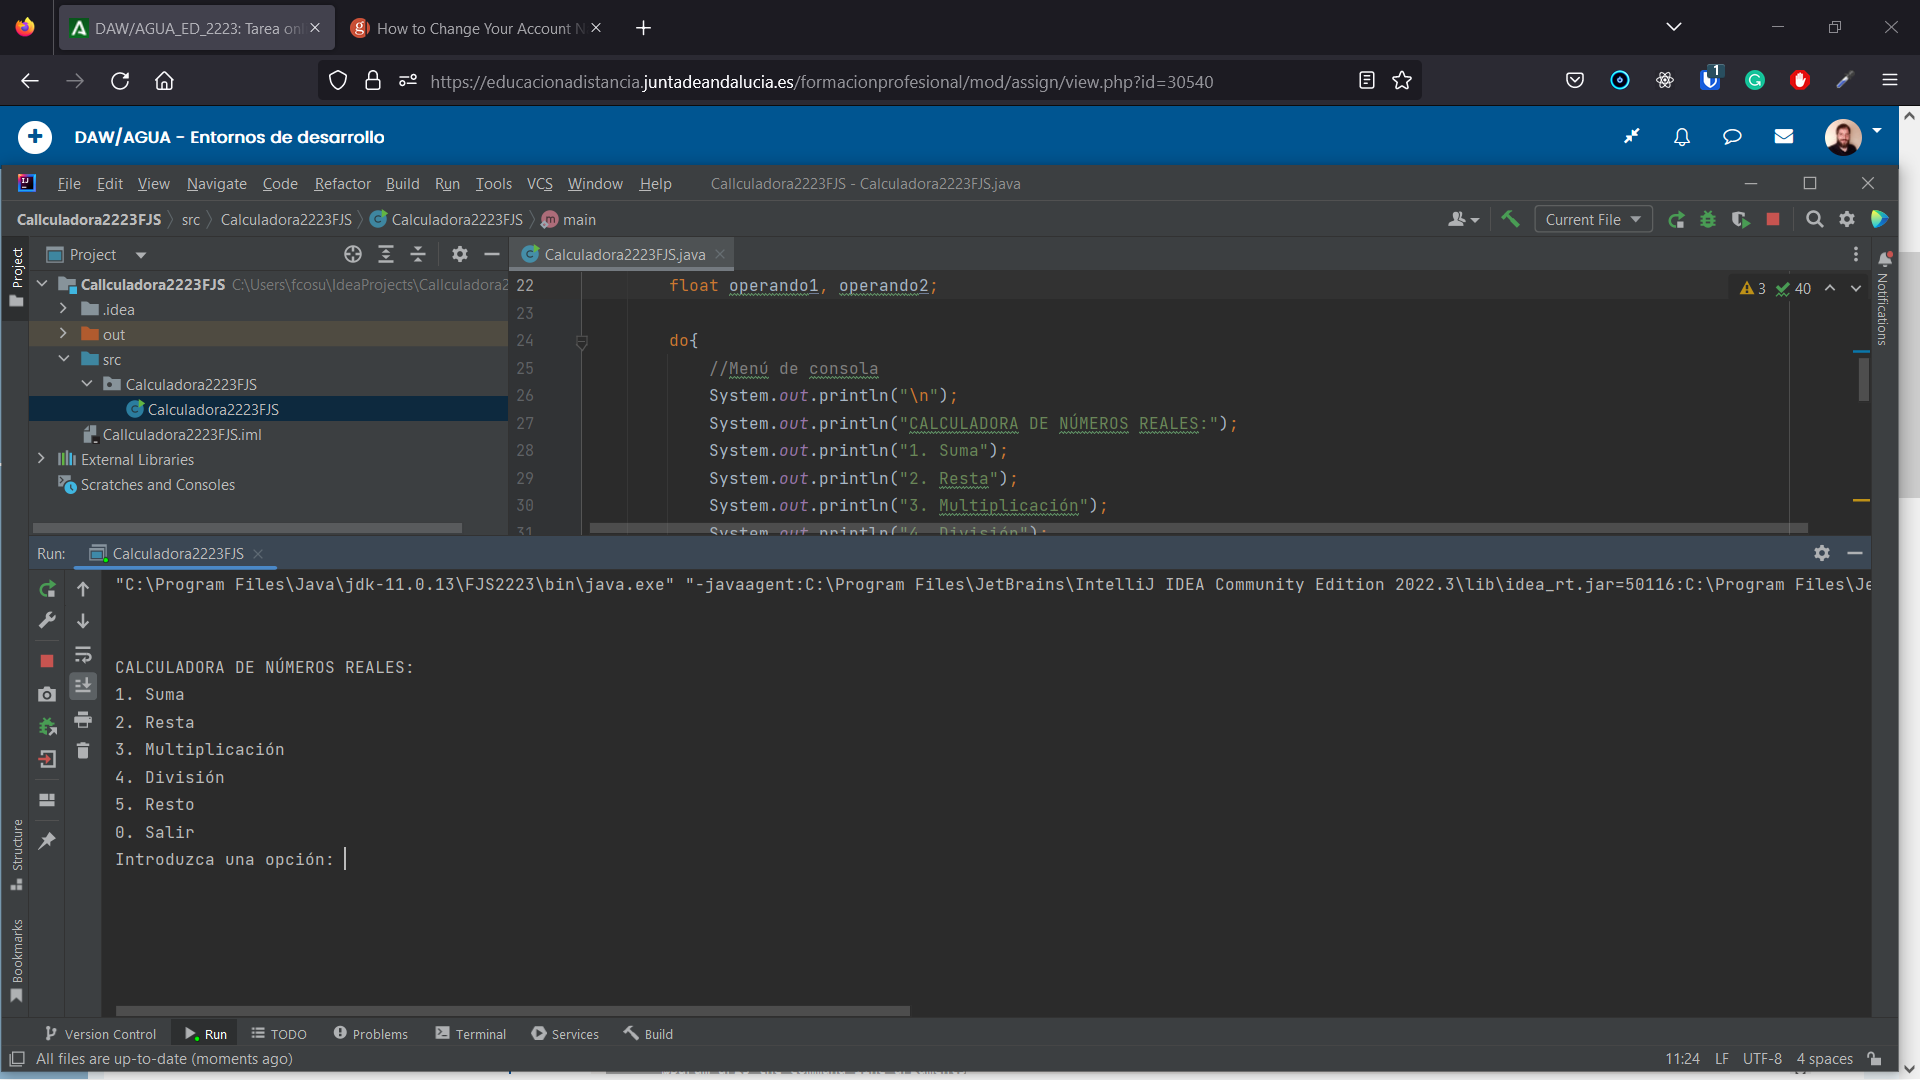
\includegraphics[scale=0.32]{idea-code-2.png}
    \caption{Código en IntelliJ corregido y ejecutado}
\end{figure}

% Bibliography

\newpage
\bibliography{citas}
\bibliographystyle{unsrt}

\end{document}